% =============================================================================
%  Dataset overview + method-comparison figures
%  Generated assets live in figures/dataset_losses/:
%    era5_lowres.png                 -- 24-channel ERA5 LowRes conditioning S_t
%    highres.png                     -- 4-channel HighRes target X_{t+1}
%    method_comparison_qpepre.png    -- truth | StormCast(EDM) | FlowCast | MeanFlow (precip)
%    method_comparison_u10.png       -- same four-way comparison for 10 m zonal wind
%
%  Scene: 2022-01-01 01:00 UTC (validation index 0); the HighRes target panel
%  is the same field shown as "truth" in the method-comparison panels.
%
%  Requires graphicx + subcaption (already loaded by the thesis preamble).
%  Include with:  % =============================================================================
%  Dataset overview + method-comparison figures
%  Generated assets live in figures/dataset_losses/:
%    era5_lowres.png                 -- 24-channel ERA5 LowRes conditioning S_t
%    highres.png                     -- 4-channel HighRes target X_{t+1}
%    method_comparison_qpepre.png    -- truth | StormCast(EDM) | FlowCast | MeanFlow (precip)
%    method_comparison_u10.png       -- same four-way comparison for 10 m zonal wind
%
%  Scene: 2022-01-01 01:00 UTC (validation index 0); the HighRes target panel
%  is the same field shown as "truth" in the method-comparison panels.
%
%  Requires graphicx + subcaption (already loaded by the thesis preamble).
%  Include with:  % =============================================================================
%  Dataset overview + method-comparison figures
%  Generated assets live in figures/dataset_losses/:
%    era5_lowres.png                 -- 24-channel ERA5 LowRes conditioning S_t
%    highres.png                     -- 4-channel HighRes target X_{t+1}
%    method_comparison_qpepre.png    -- truth | StormCast(EDM) | FlowCast | MeanFlow (precip)
%    method_comparison_u10.png       -- same four-way comparison for 10 m zonal wind
%
%  Scene: 2022-01-01 01:00 UTC (validation index 0); the HighRes target panel
%  is the same field shown as "truth" in the method-comparison panels.
%
%  Requires graphicx + subcaption (already loaded by the thesis preamble).
%  Include with:  % =============================================================================
%  Dataset overview + method-comparison figures
%  Generated assets live in figures/dataset_losses/:
%    era5_lowres.png                 -- 24-channel ERA5 LowRes conditioning S_t
%    highres.png                     -- 4-channel HighRes target X_{t+1}
%    method_comparison_qpepre.png    -- truth | StormCast(EDM) | FlowCast | MeanFlow (precip)
%    method_comparison_u10.png       -- same four-way comparison for 10 m zonal wind
%
%  Scene: 2022-01-01 01:00 UTC (validation index 0); the HighRes target panel
%  is the same field shown as "truth" in the method-comparison panels.
%
%  Requires graphicx + subcaption (already loaded by the thesis preamble).
%  Include with:  \input{figures/dataset_losses/dataset_losses.tex}
% =============================================================================

% -----------------------------------------------------------------------------
% 1. ERA5 LowRes conditioning input S_t
% -----------------------------------------------------------------------------
\begin{figure}[htbp]
  \centering
  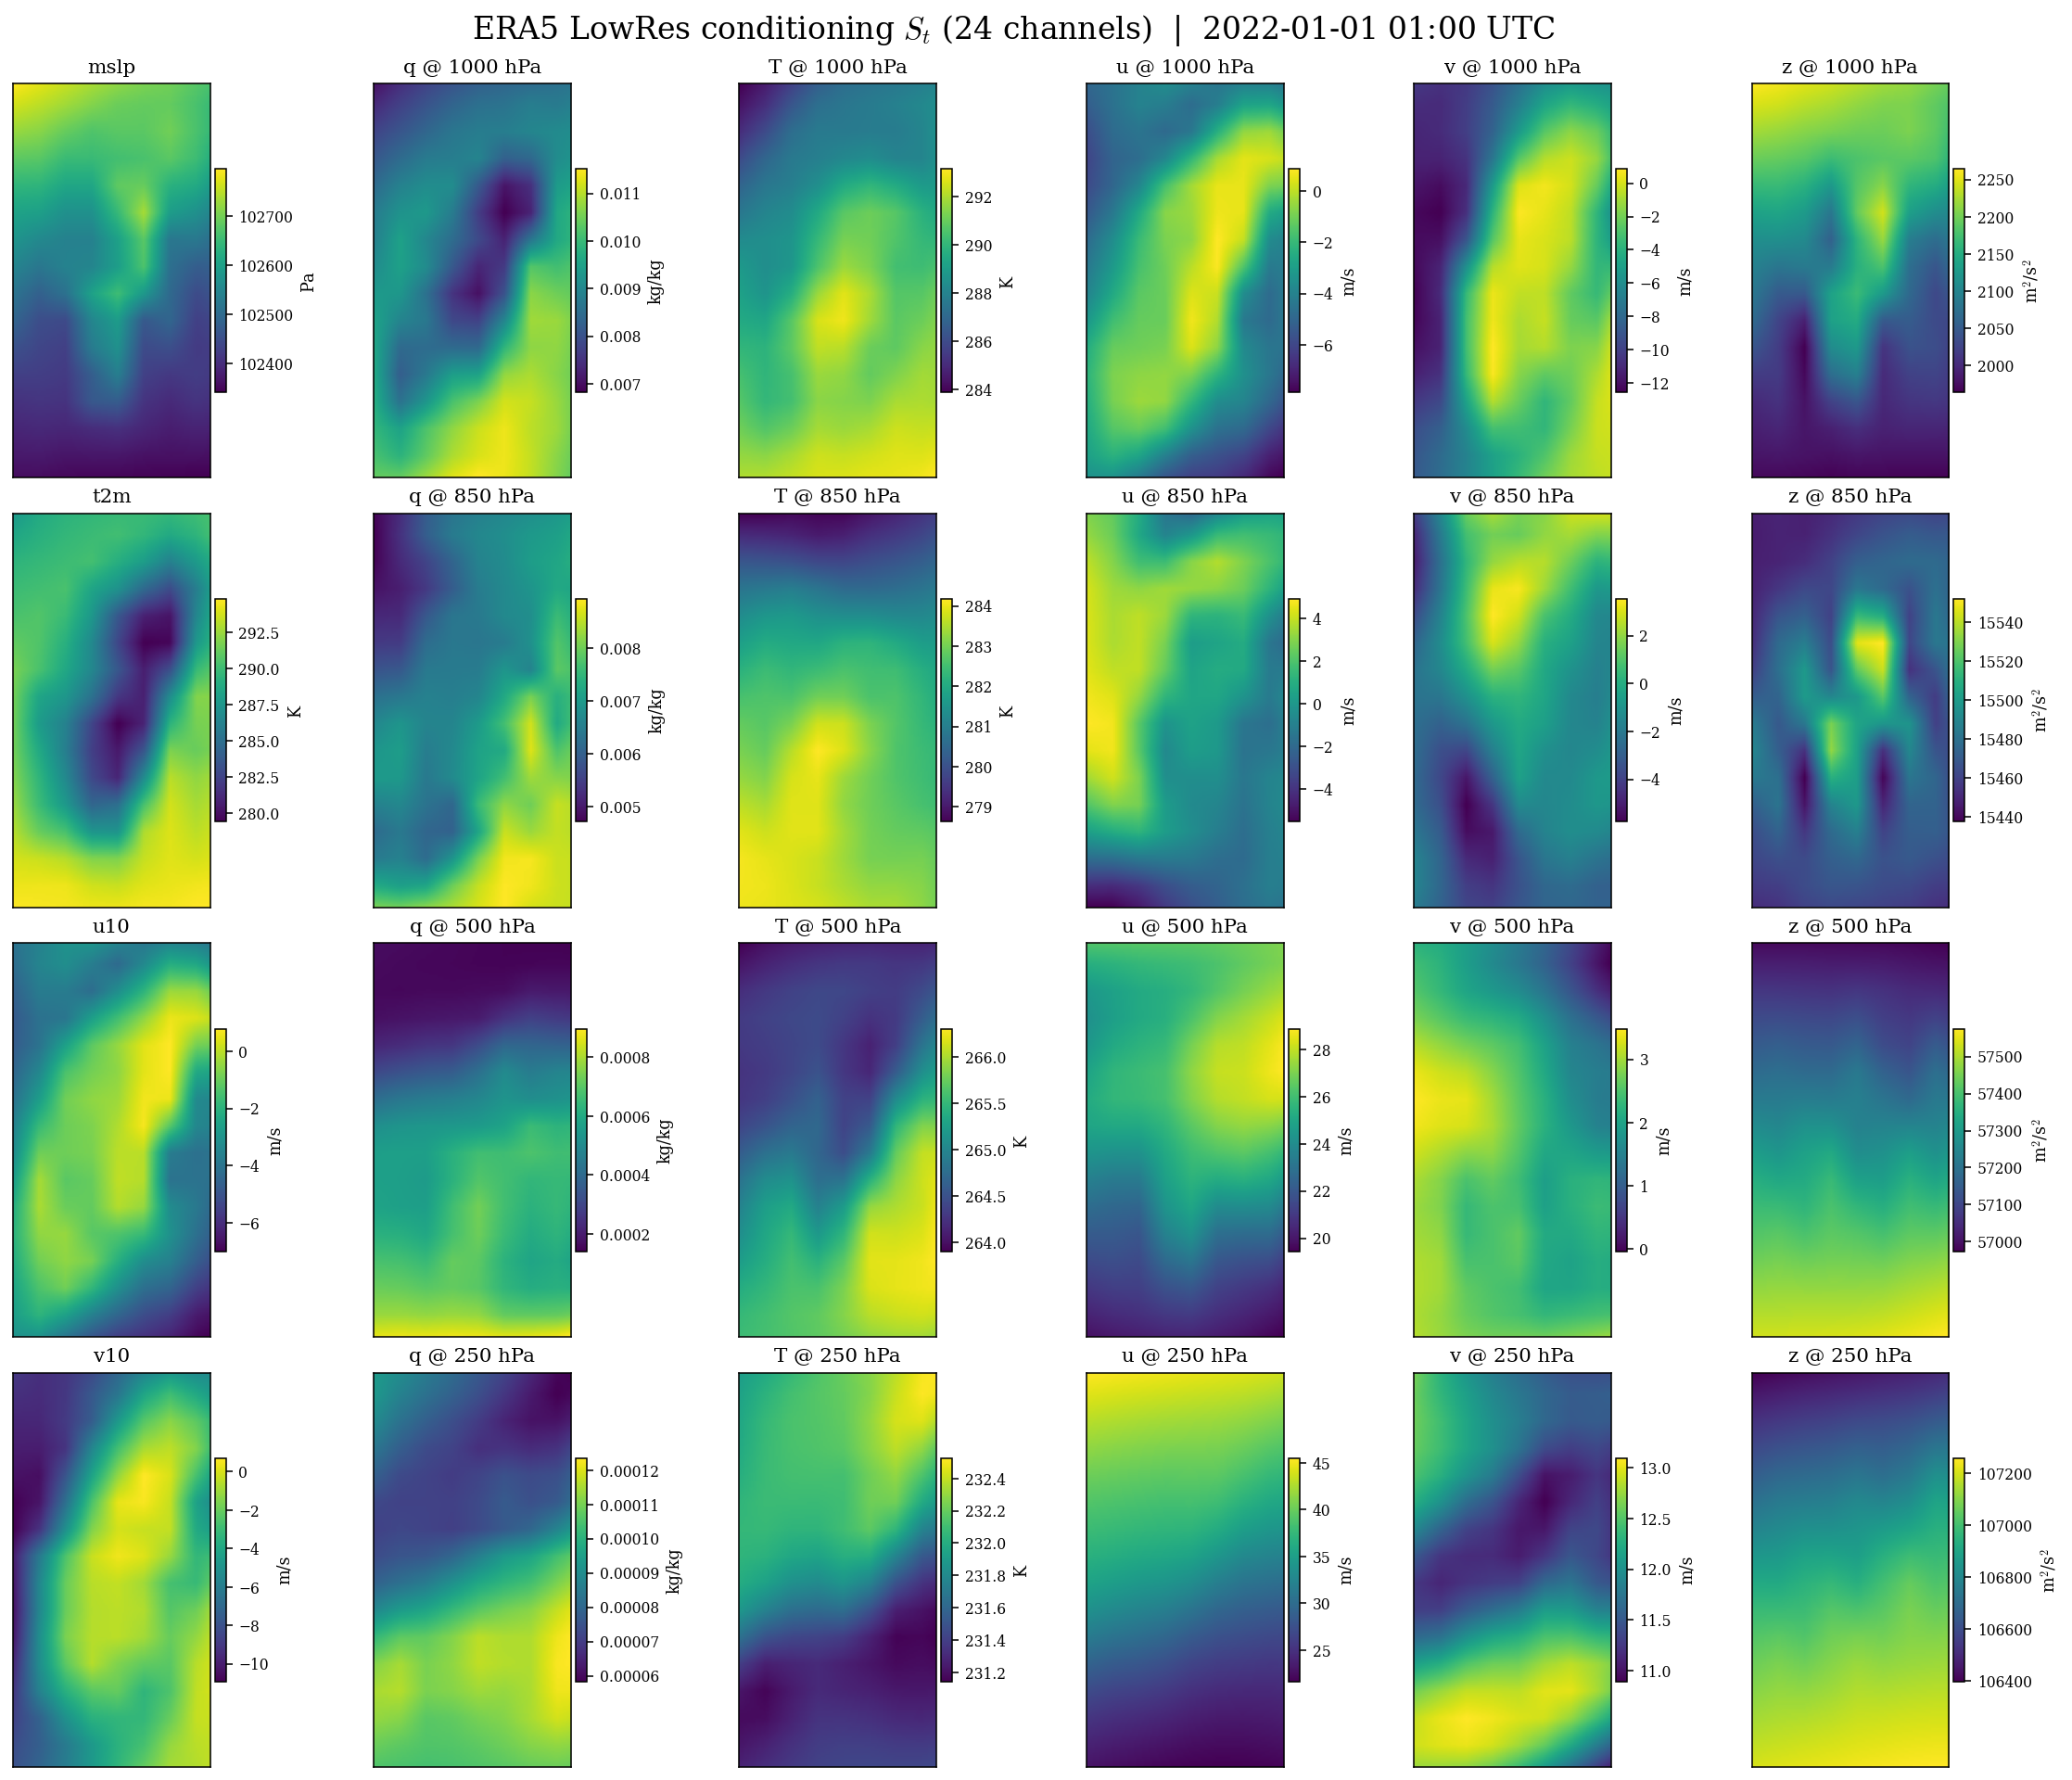
\includegraphics[width=\linewidth]{figures/dataset_losses/era5_lowres.png}
  \caption[ERA5 LowRes conditioning input]{The 24-channel ERA5 LowRes
  conditioning state $S_t$ for a single validation hour (2022-01-01 01:00 UTC),
  in physical units. Top row: the four surface variables (mean sea-level
  pressure, two-metre temperature, ten-metre zonal and meridional winds).
  Rows two through six: specific humidity $q$, temperature $T$, and the wind
  components $u$, $v$ together with geopotential height $z$, each shown across
  the four standard pressure levels \SIlist{1000;850;500;250}{\hecto\pascal}.
  These coarse ($\sim$\SI{25}{\kilo\metre}) re-gridded reanalysis fields supply
  the synoptic-scale environment; they enter the residual heads only indirectly,
  through the regression mean. All panels use the \texttt{viridis} colormap with
  per-panel colour limits. Generated by
  \texttt{experiment\_scripts/make\_dataset\_overview\_figures.py}.}
  \label{fig:era5-lowres}
\end{figure}

% -----------------------------------------------------------------------------
% 2. HighRes target X_{t+1}
% -----------------------------------------------------------------------------
\begin{figure}[htbp]
  \centering
  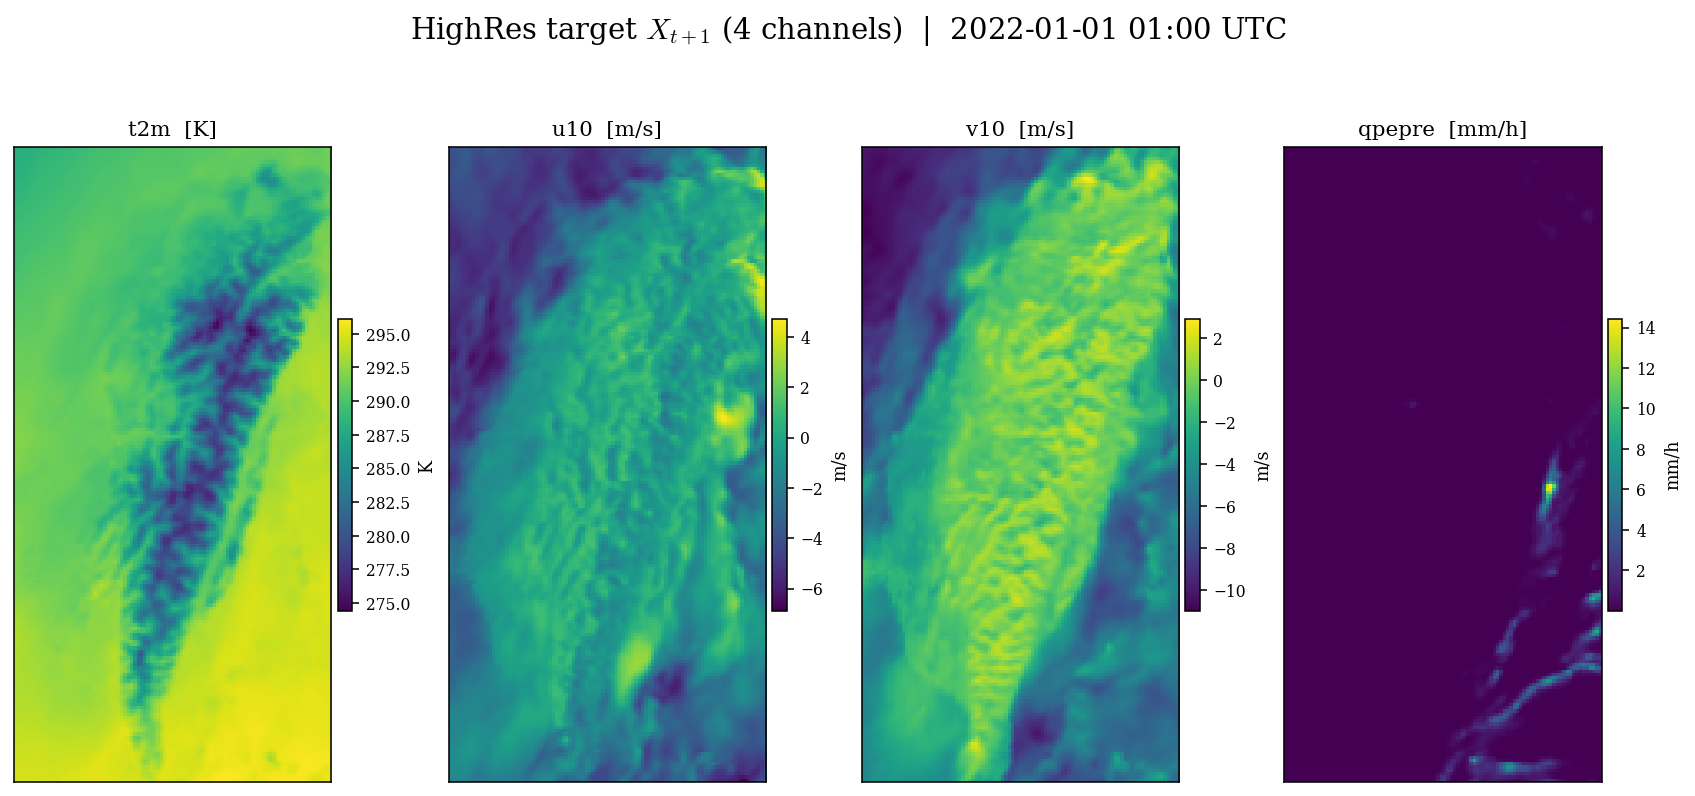
\includegraphics[width=\linewidth]{figures/dataset_losses/highres.png}
  \caption[HighRes target fields]{The four-channel HighRes target $X_{t+1}$ for
  the same validation hour as Figure~\ref{fig:era5-lowres}: two-metre
  temperature \texttt{t2m} (K), ten-metre winds \texttt{u10}, \texttt{v10}
  (m\,s$^{-1}$), and radar-derived hourly precipitation \texttt{qpepre}
  (mm\,h$^{-1}$). The convection-permitting $\sim$\SI{2}{\kilo\metre} grid
  resolves Taiwan's Central Mountain Range (visible as the cold spine in
  \texttt{t2m}) and the sparse, sharp-edged precipitation field that makes
  \texttt{qpepre} the hard channel. This \texttt{qpepre} field is the same one
  shown as ``truth'' in Figure~\ref{fig:method-comparison}. Generated by
  \texttt{experiment\_scripts/make\_dataset\_overview\_figures.py}.}
  \label{fig:highres-target}
\end{figure}

% -----------------------------------------------------------------------------
% 3. Method comparison: StormCast (EDM) vs FlowCast vs MeanFlow
% -----------------------------------------------------------------------------
\begin{figure}[htbp]
  \centering
  \begin{subfigure}[t]{\linewidth}
    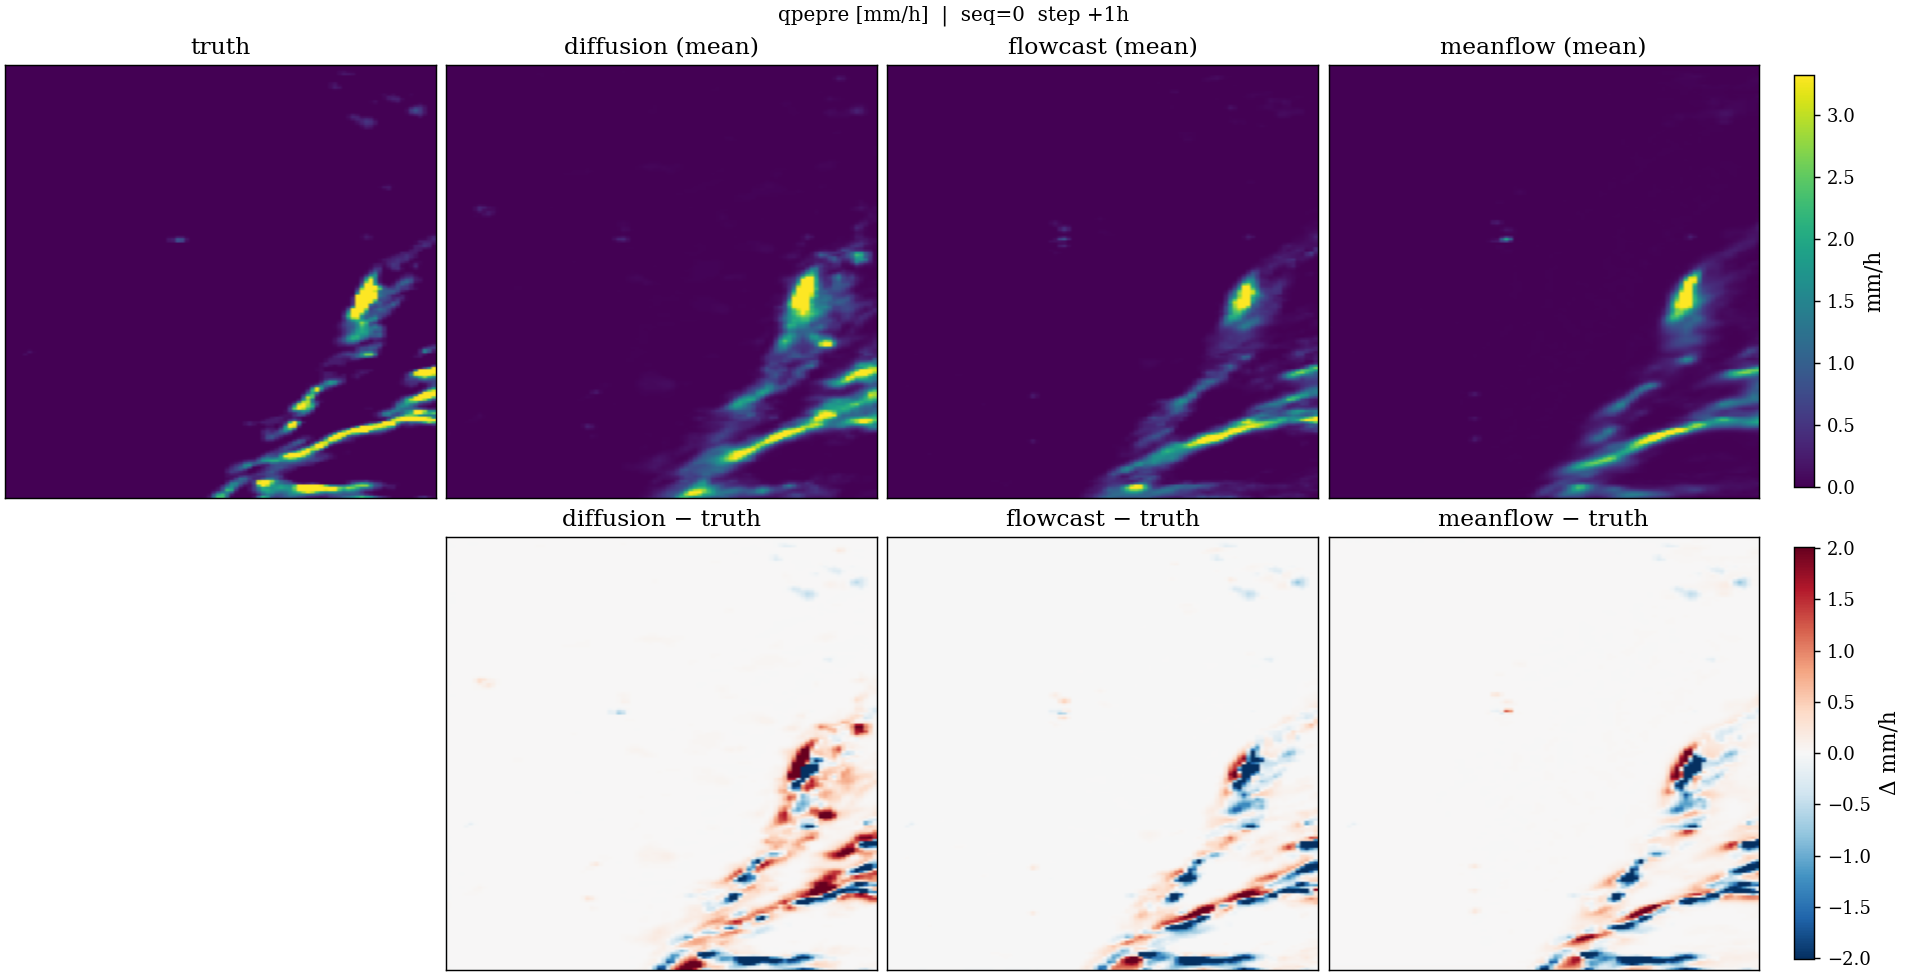
\includegraphics[width=\linewidth]{figures/dataset_losses/method_comparison_qpepre.png}
    \caption{Precipitation \texttt{qpepre} (mm\,h$^{-1}$).}
    \label{fig:method-comparison-qpepre}
  \end{subfigure}

  \vspace{0.8em}
  \begin{subfigure}[t]{\linewidth}
    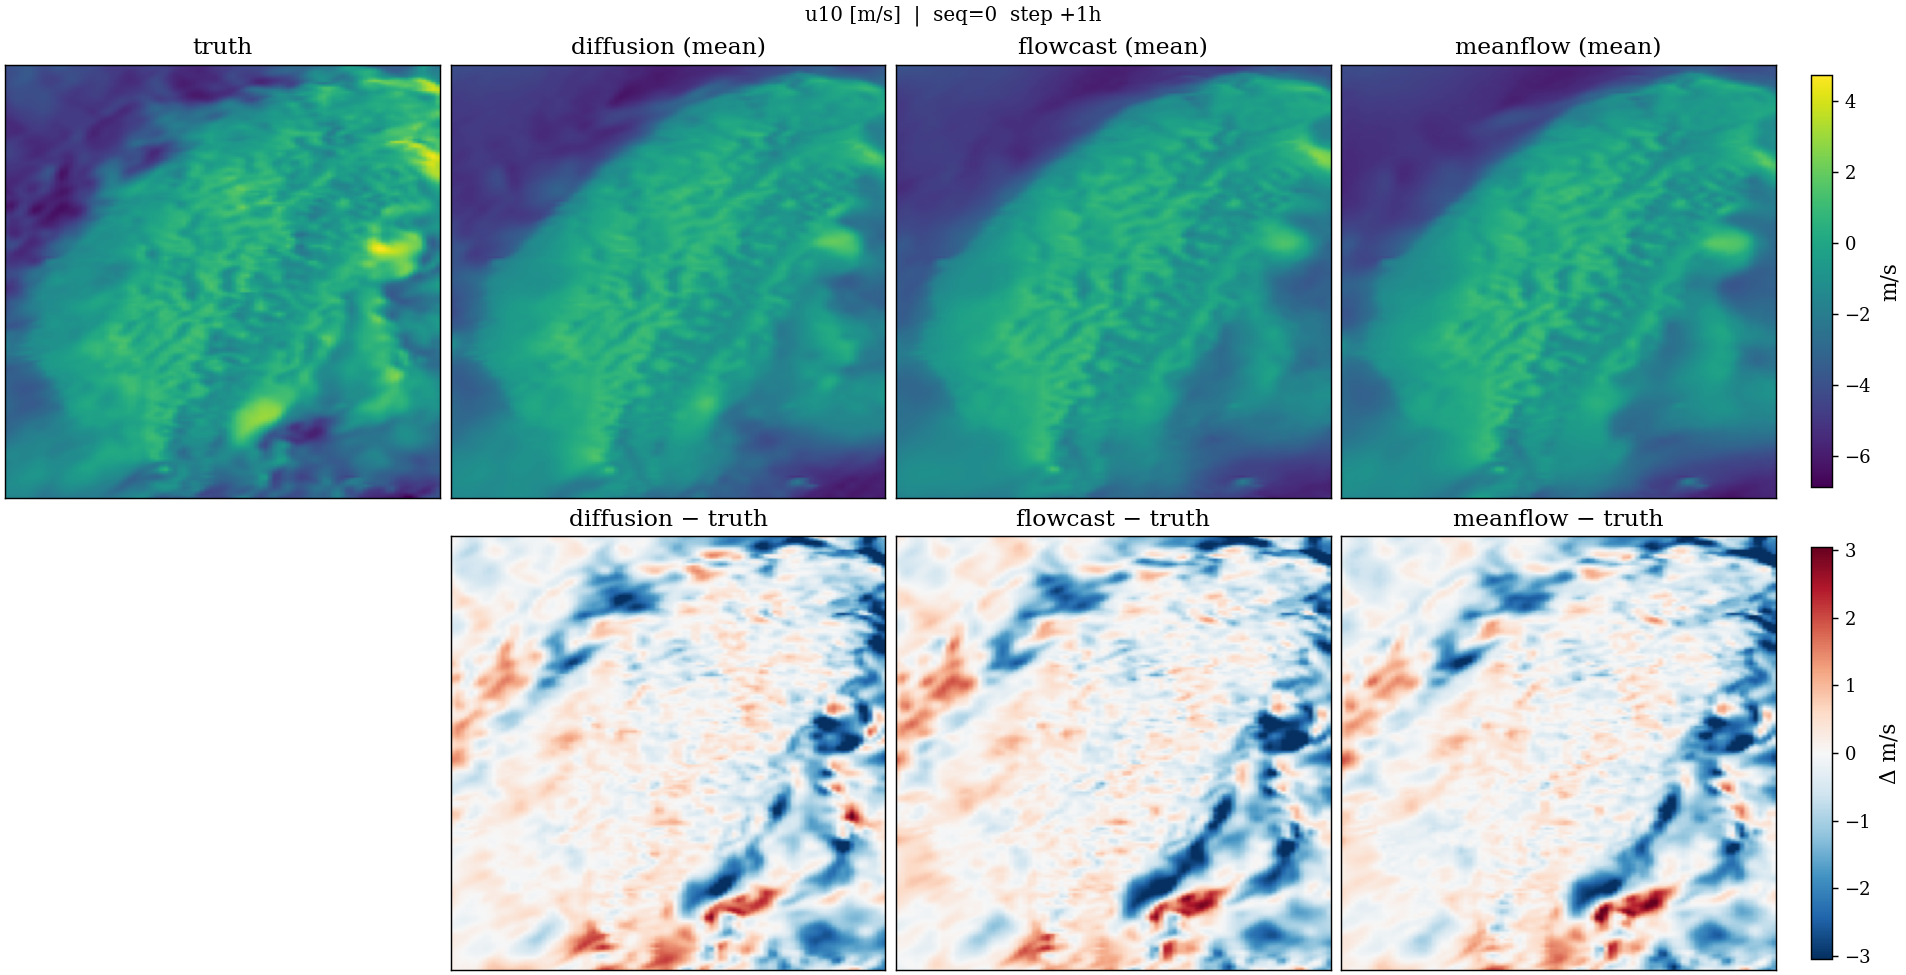
\includegraphics[width=\linewidth]{figures/dataset_losses/method_comparison_u10.png}
    \caption{Ten-metre zonal wind \texttt{u10} (m\,s$^{-1}$).}
    \label{fig:method-comparison-u10}
  \end{subfigure}
  \caption[Qualitative comparison of the three generative heads]{Qualitative
  head-to-head comparison of the three generative residual methods on the
  same +1\,h validation step (2022-01-01 01:00 UTC). In each panel the top row
  shows, left to right, the RWRF/QPEPRE ground truth and the 10-member ensemble
  means of StormCast (the EDM diffusion teacher, labelled \emph{diffusion}),
  FlowCast (CFM student), and MeanFlow (average-velocity student, 1--2 NFE); the
  bottom row shows the corresponding signed error fields (prediction $-$ truth)
  on a diverging scale. All three heads condition on the identical regression
  mean $M_t$, so any difference is attributable to the generative trajectory
  alone. StormCast is the original diffusion baseline; FlowCast and MeanFlow are
  the flow-matching students that match or beat it at a fraction of the
  sampling cost. Field panels use \texttt{viridis}; difference panels use a
  symmetric \texttt{RdBu\_r} scale centred on zero. Generated by
  \texttt{experiment\_scripts/compare\_diffusion\_vs\_flowcast.py}.}
  \label{fig:method-comparison}
\end{figure}

% =============================================================================

% -----------------------------------------------------------------------------
% 1. ERA5 LowRes conditioning input S_t
% -----------------------------------------------------------------------------
\begin{figure}[htbp]
  \centering
  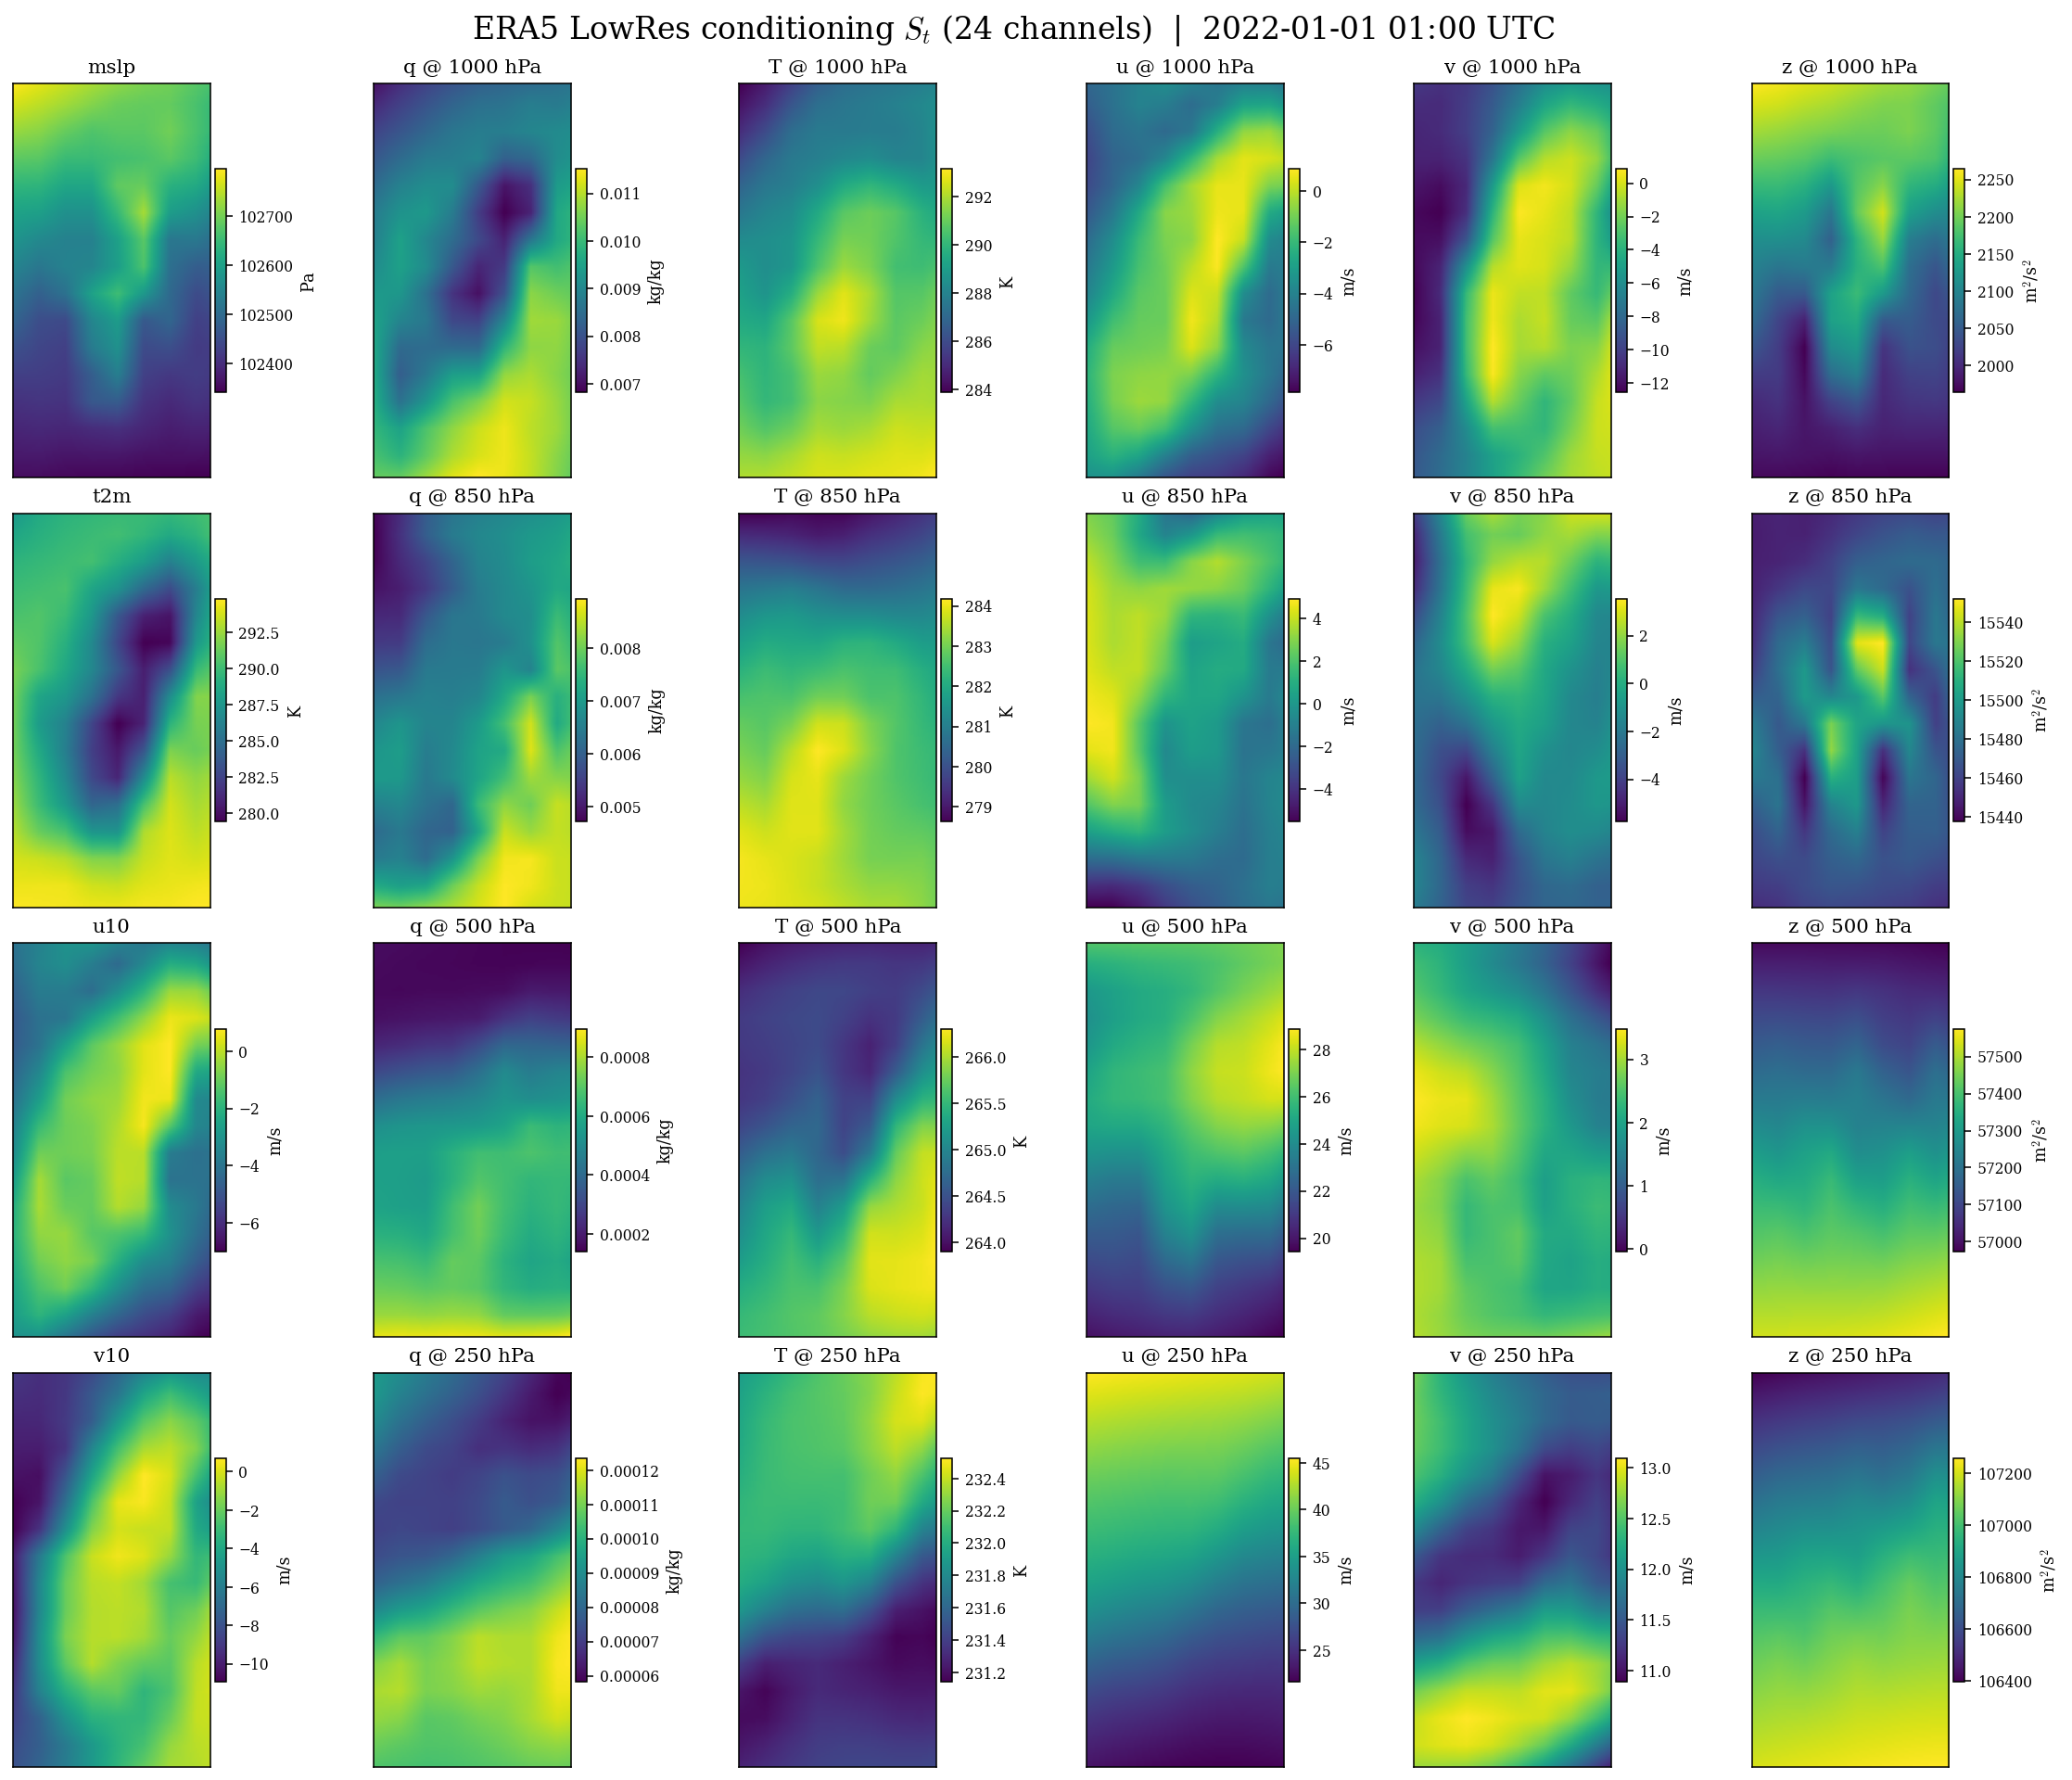
\includegraphics[width=\linewidth]{figures/dataset_losses/era5_lowres.png}
  \caption[ERA5 LowRes conditioning input]{The 24-channel ERA5 LowRes
  conditioning state $S_t$ for a single validation hour (2022-01-01 01:00 UTC),
  in physical units. Top row: the four surface variables (mean sea-level
  pressure, two-metre temperature, ten-metre zonal and meridional winds).
  Rows two through six: specific humidity $q$, temperature $T$, and the wind
  components $u$, $v$ together with geopotential height $z$, each shown across
  the four standard pressure levels \SIlist{1000;850;500;250}{\hecto\pascal}.
  These coarse ($\sim$\SI{25}{\kilo\metre}) re-gridded reanalysis fields supply
  the synoptic-scale environment; they enter the residual heads only indirectly,
  through the regression mean. All panels use the \texttt{viridis} colormap with
  per-panel colour limits. Generated by
  \texttt{experiment\_scripts/make\_dataset\_overview\_figures.py}.}
  \label{fig:era5-lowres}
\end{figure}

% -----------------------------------------------------------------------------
% 2. HighRes target X_{t+1}
% -----------------------------------------------------------------------------
\begin{figure}[htbp]
  \centering
  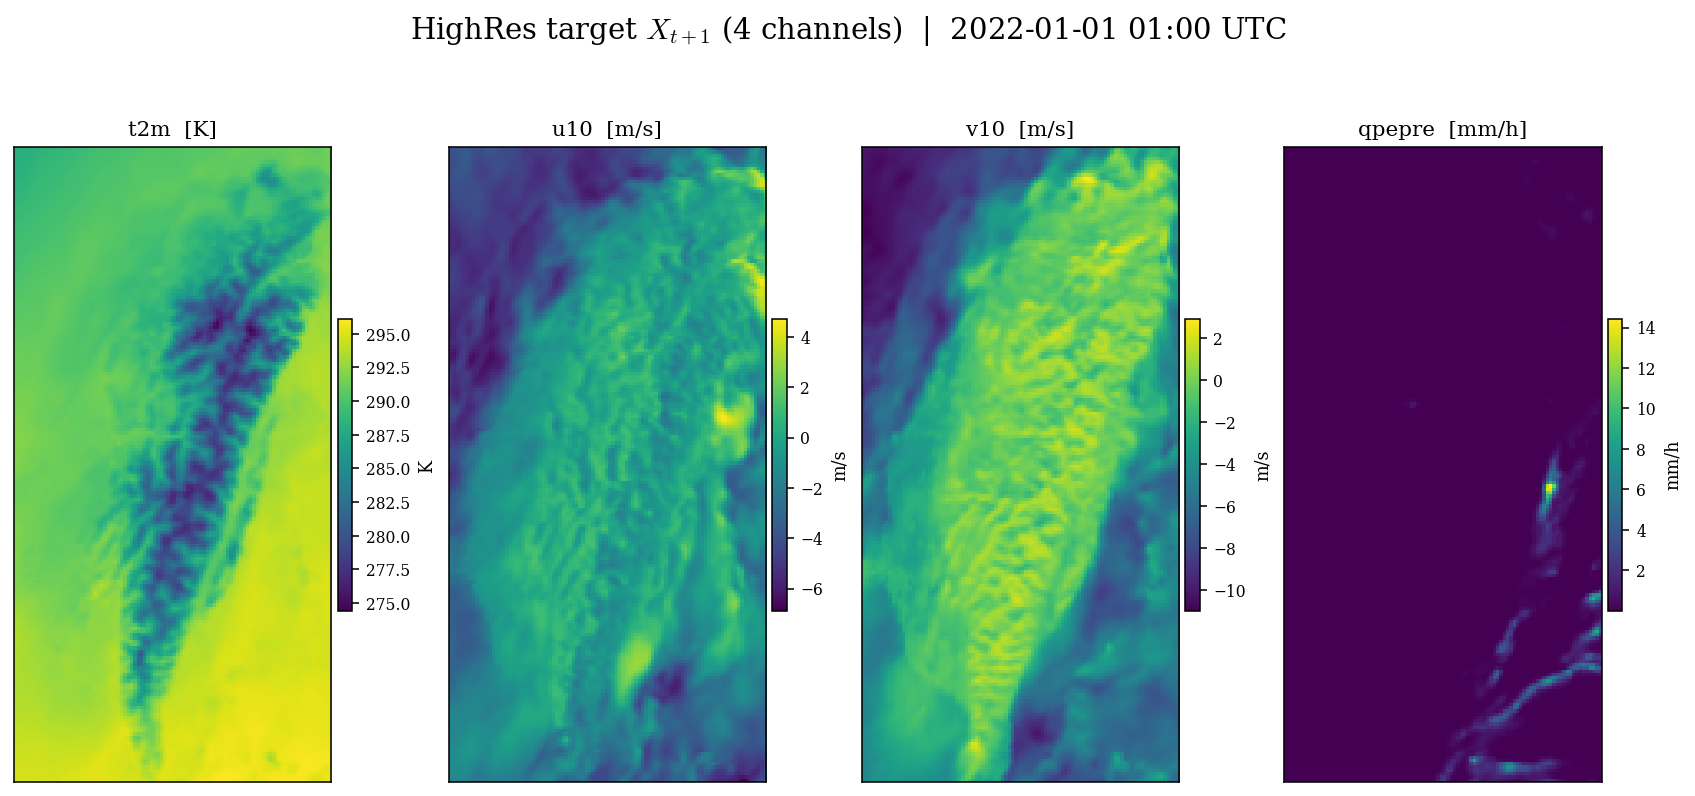
\includegraphics[width=\linewidth]{figures/dataset_losses/highres.png}
  \caption[HighRes target fields]{The four-channel HighRes target $X_{t+1}$ for
  the same validation hour as Figure~\ref{fig:era5-lowres}: two-metre
  temperature \texttt{t2m} (K), ten-metre winds \texttt{u10}, \texttt{v10}
  (m\,s$^{-1}$), and radar-derived hourly precipitation \texttt{qpepre}
  (mm\,h$^{-1}$). The convection-permitting $\sim$\SI{2}{\kilo\metre} grid
  resolves Taiwan's Central Mountain Range (visible as the cold spine in
  \texttt{t2m}) and the sparse, sharp-edged precipitation field that makes
  \texttt{qpepre} the hard channel. This \texttt{qpepre} field is the same one
  shown as ``truth'' in Figure~\ref{fig:method-comparison}. Generated by
  \texttt{experiment\_scripts/make\_dataset\_overview\_figures.py}.}
  \label{fig:highres-target}
\end{figure}

% -----------------------------------------------------------------------------
% 3. Method comparison: StormCast (EDM) vs FlowCast vs MeanFlow
% -----------------------------------------------------------------------------
\begin{figure}[htbp]
  \centering
  \begin{subfigure}[t]{\linewidth}
    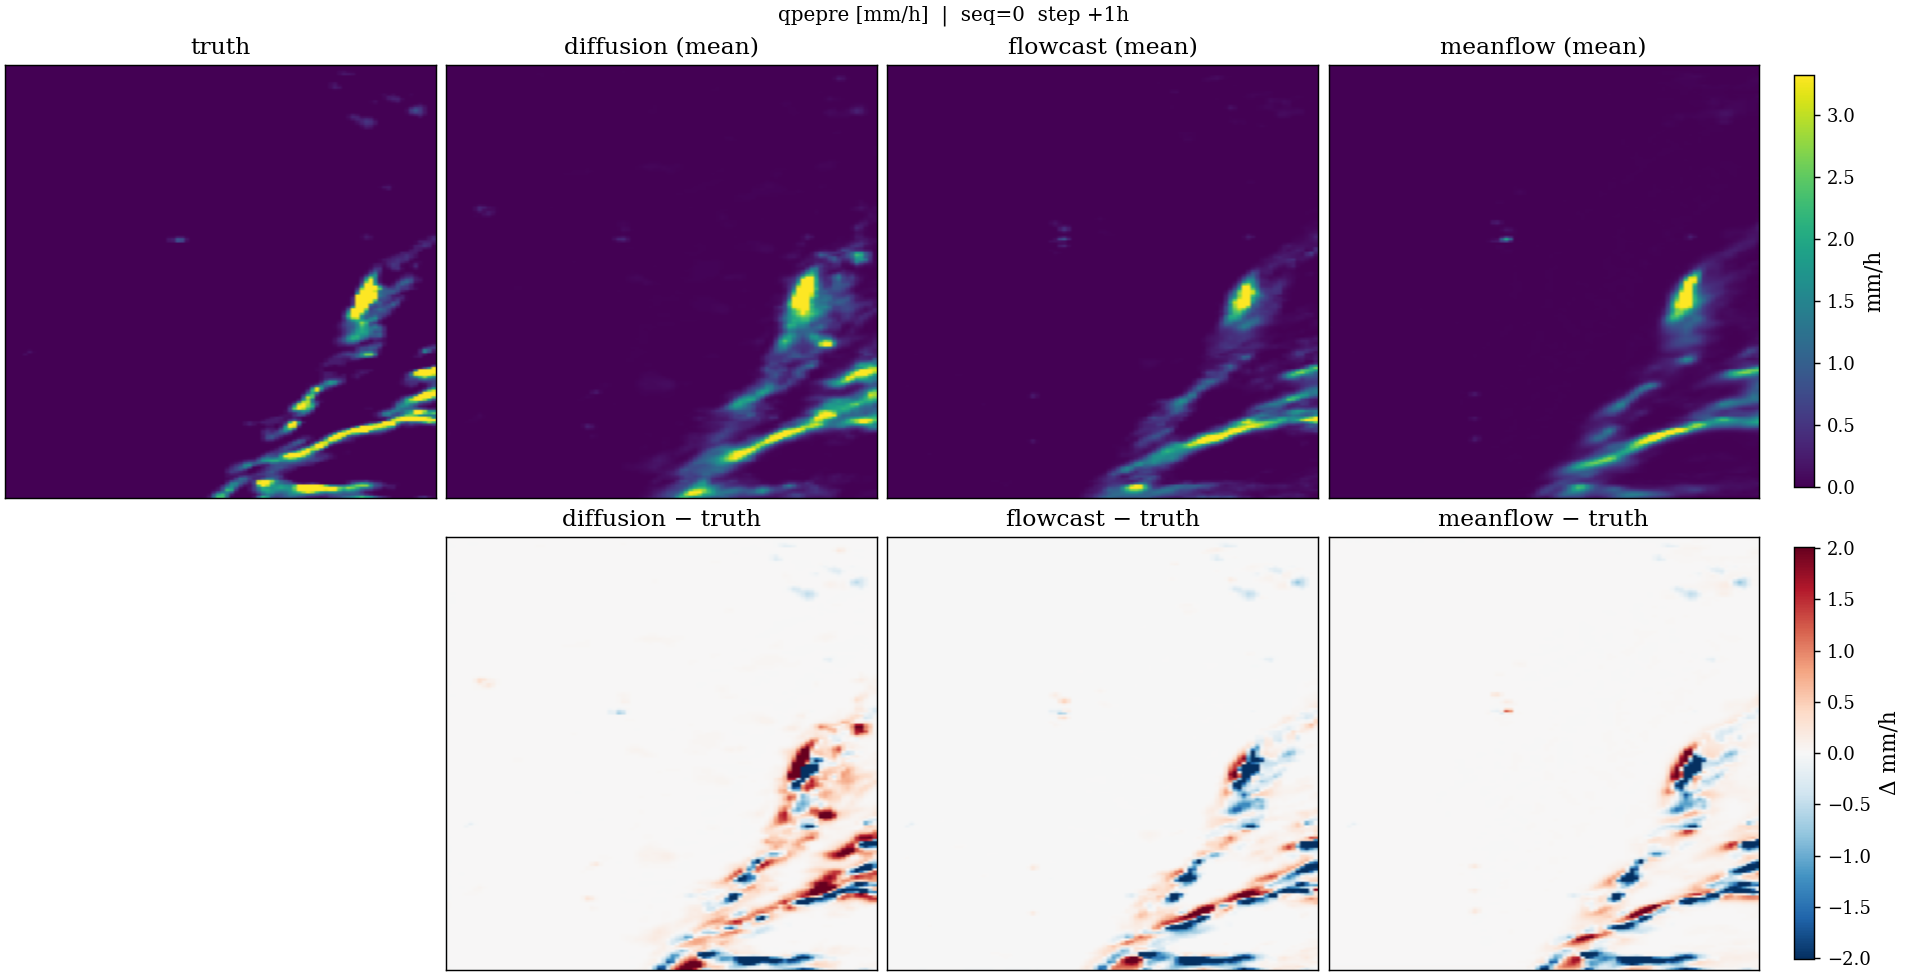
\includegraphics[width=\linewidth]{figures/dataset_losses/method_comparison_qpepre.png}
    \caption{Precipitation \texttt{qpepre} (mm\,h$^{-1}$).}
    \label{fig:method-comparison-qpepre}
  \end{subfigure}

  \vspace{0.8em}
  \begin{subfigure}[t]{\linewidth}
    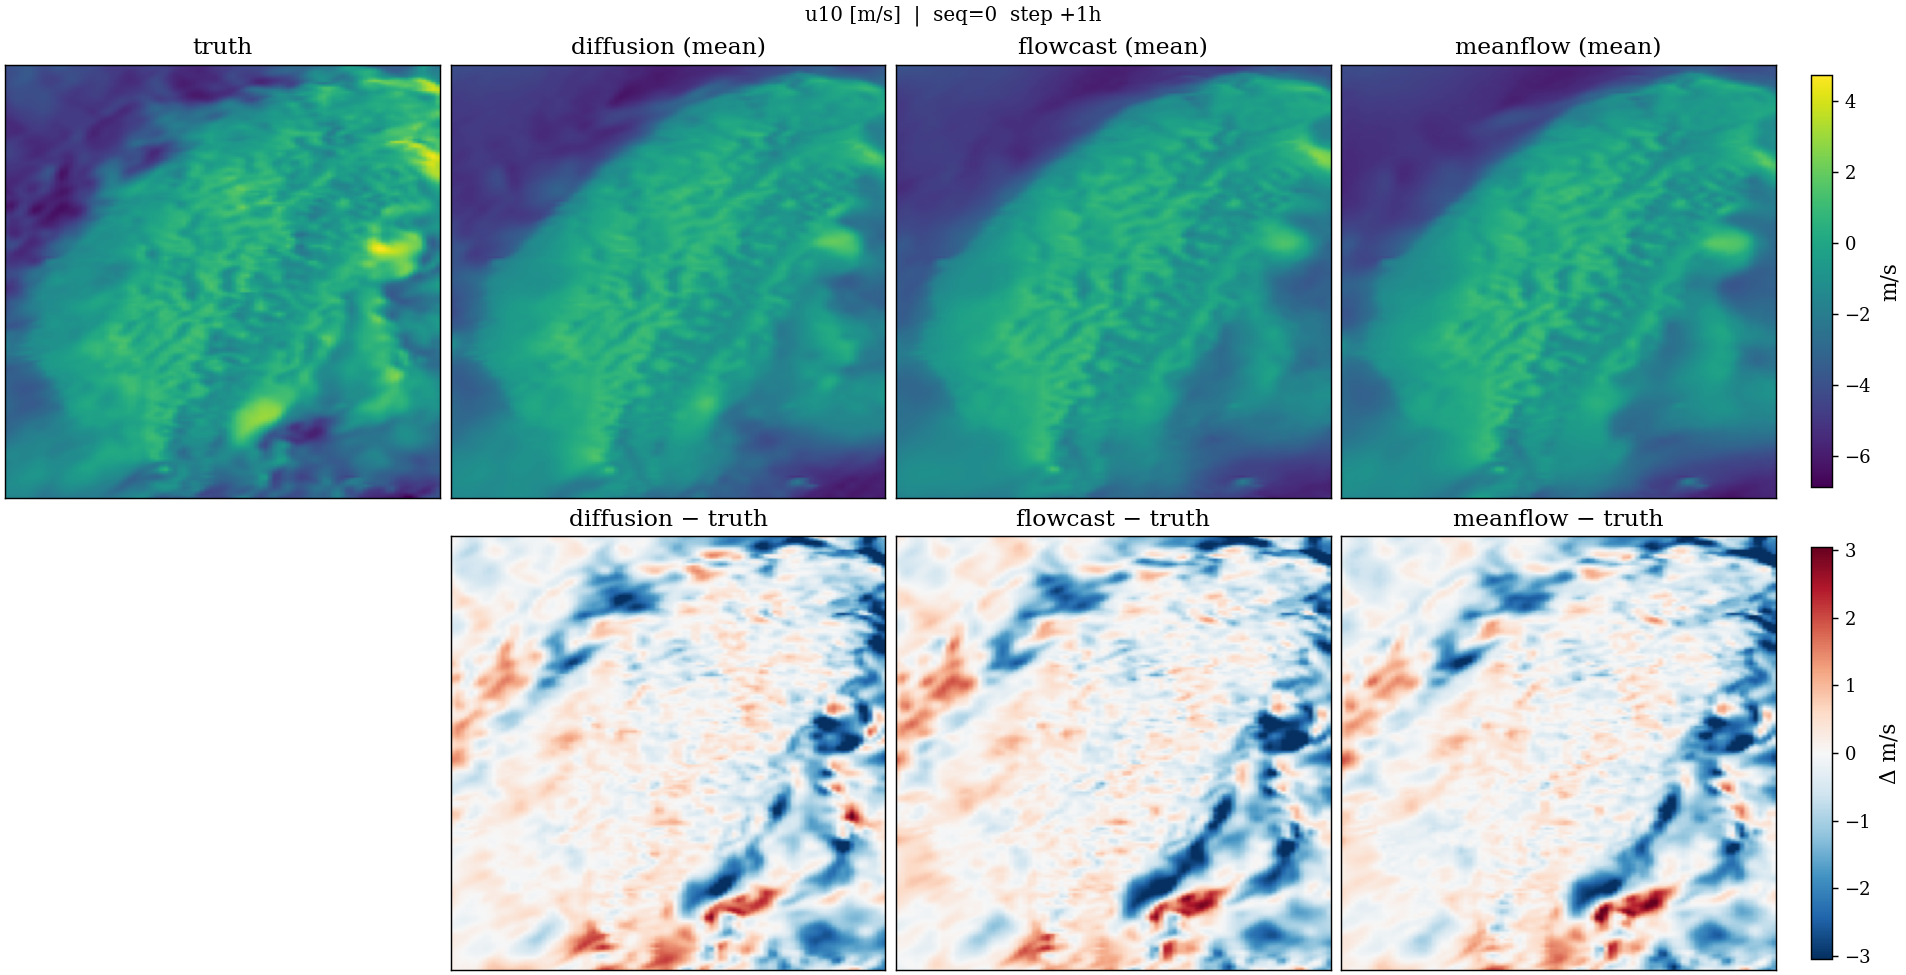
\includegraphics[width=\linewidth]{figures/dataset_losses/method_comparison_u10.png}
    \caption{Ten-metre zonal wind \texttt{u10} (m\,s$^{-1}$).}
    \label{fig:method-comparison-u10}
  \end{subfigure}
  \caption[Qualitative comparison of the three generative heads]{Qualitative
  head-to-head comparison of the three generative residual methods on the
  same +1\,h validation step (2022-01-01 01:00 UTC). In each panel the top row
  shows, left to right, the RWRF/QPEPRE ground truth and the 10-member ensemble
  means of StormCast (the EDM diffusion teacher, labelled \emph{diffusion}),
  FlowCast (CFM student), and MeanFlow (average-velocity student, 1--2 NFE); the
  bottom row shows the corresponding signed error fields (prediction $-$ truth)
  on a diverging scale. All three heads condition on the identical regression
  mean $M_t$, so any difference is attributable to the generative trajectory
  alone. StormCast is the original diffusion baseline; FlowCast and MeanFlow are
  the flow-matching students that match or beat it at a fraction of the
  sampling cost. Field panels use \texttt{viridis}; difference panels use a
  symmetric \texttt{RdBu\_r} scale centred on zero. Generated by
  \texttt{experiment\_scripts/compare\_diffusion\_vs\_flowcast.py}.}
  \label{fig:method-comparison}
\end{figure}

% =============================================================================

% -----------------------------------------------------------------------------
% 1. ERA5 LowRes conditioning input S_t
% -----------------------------------------------------------------------------
\begin{figure}[htbp]
  \centering
  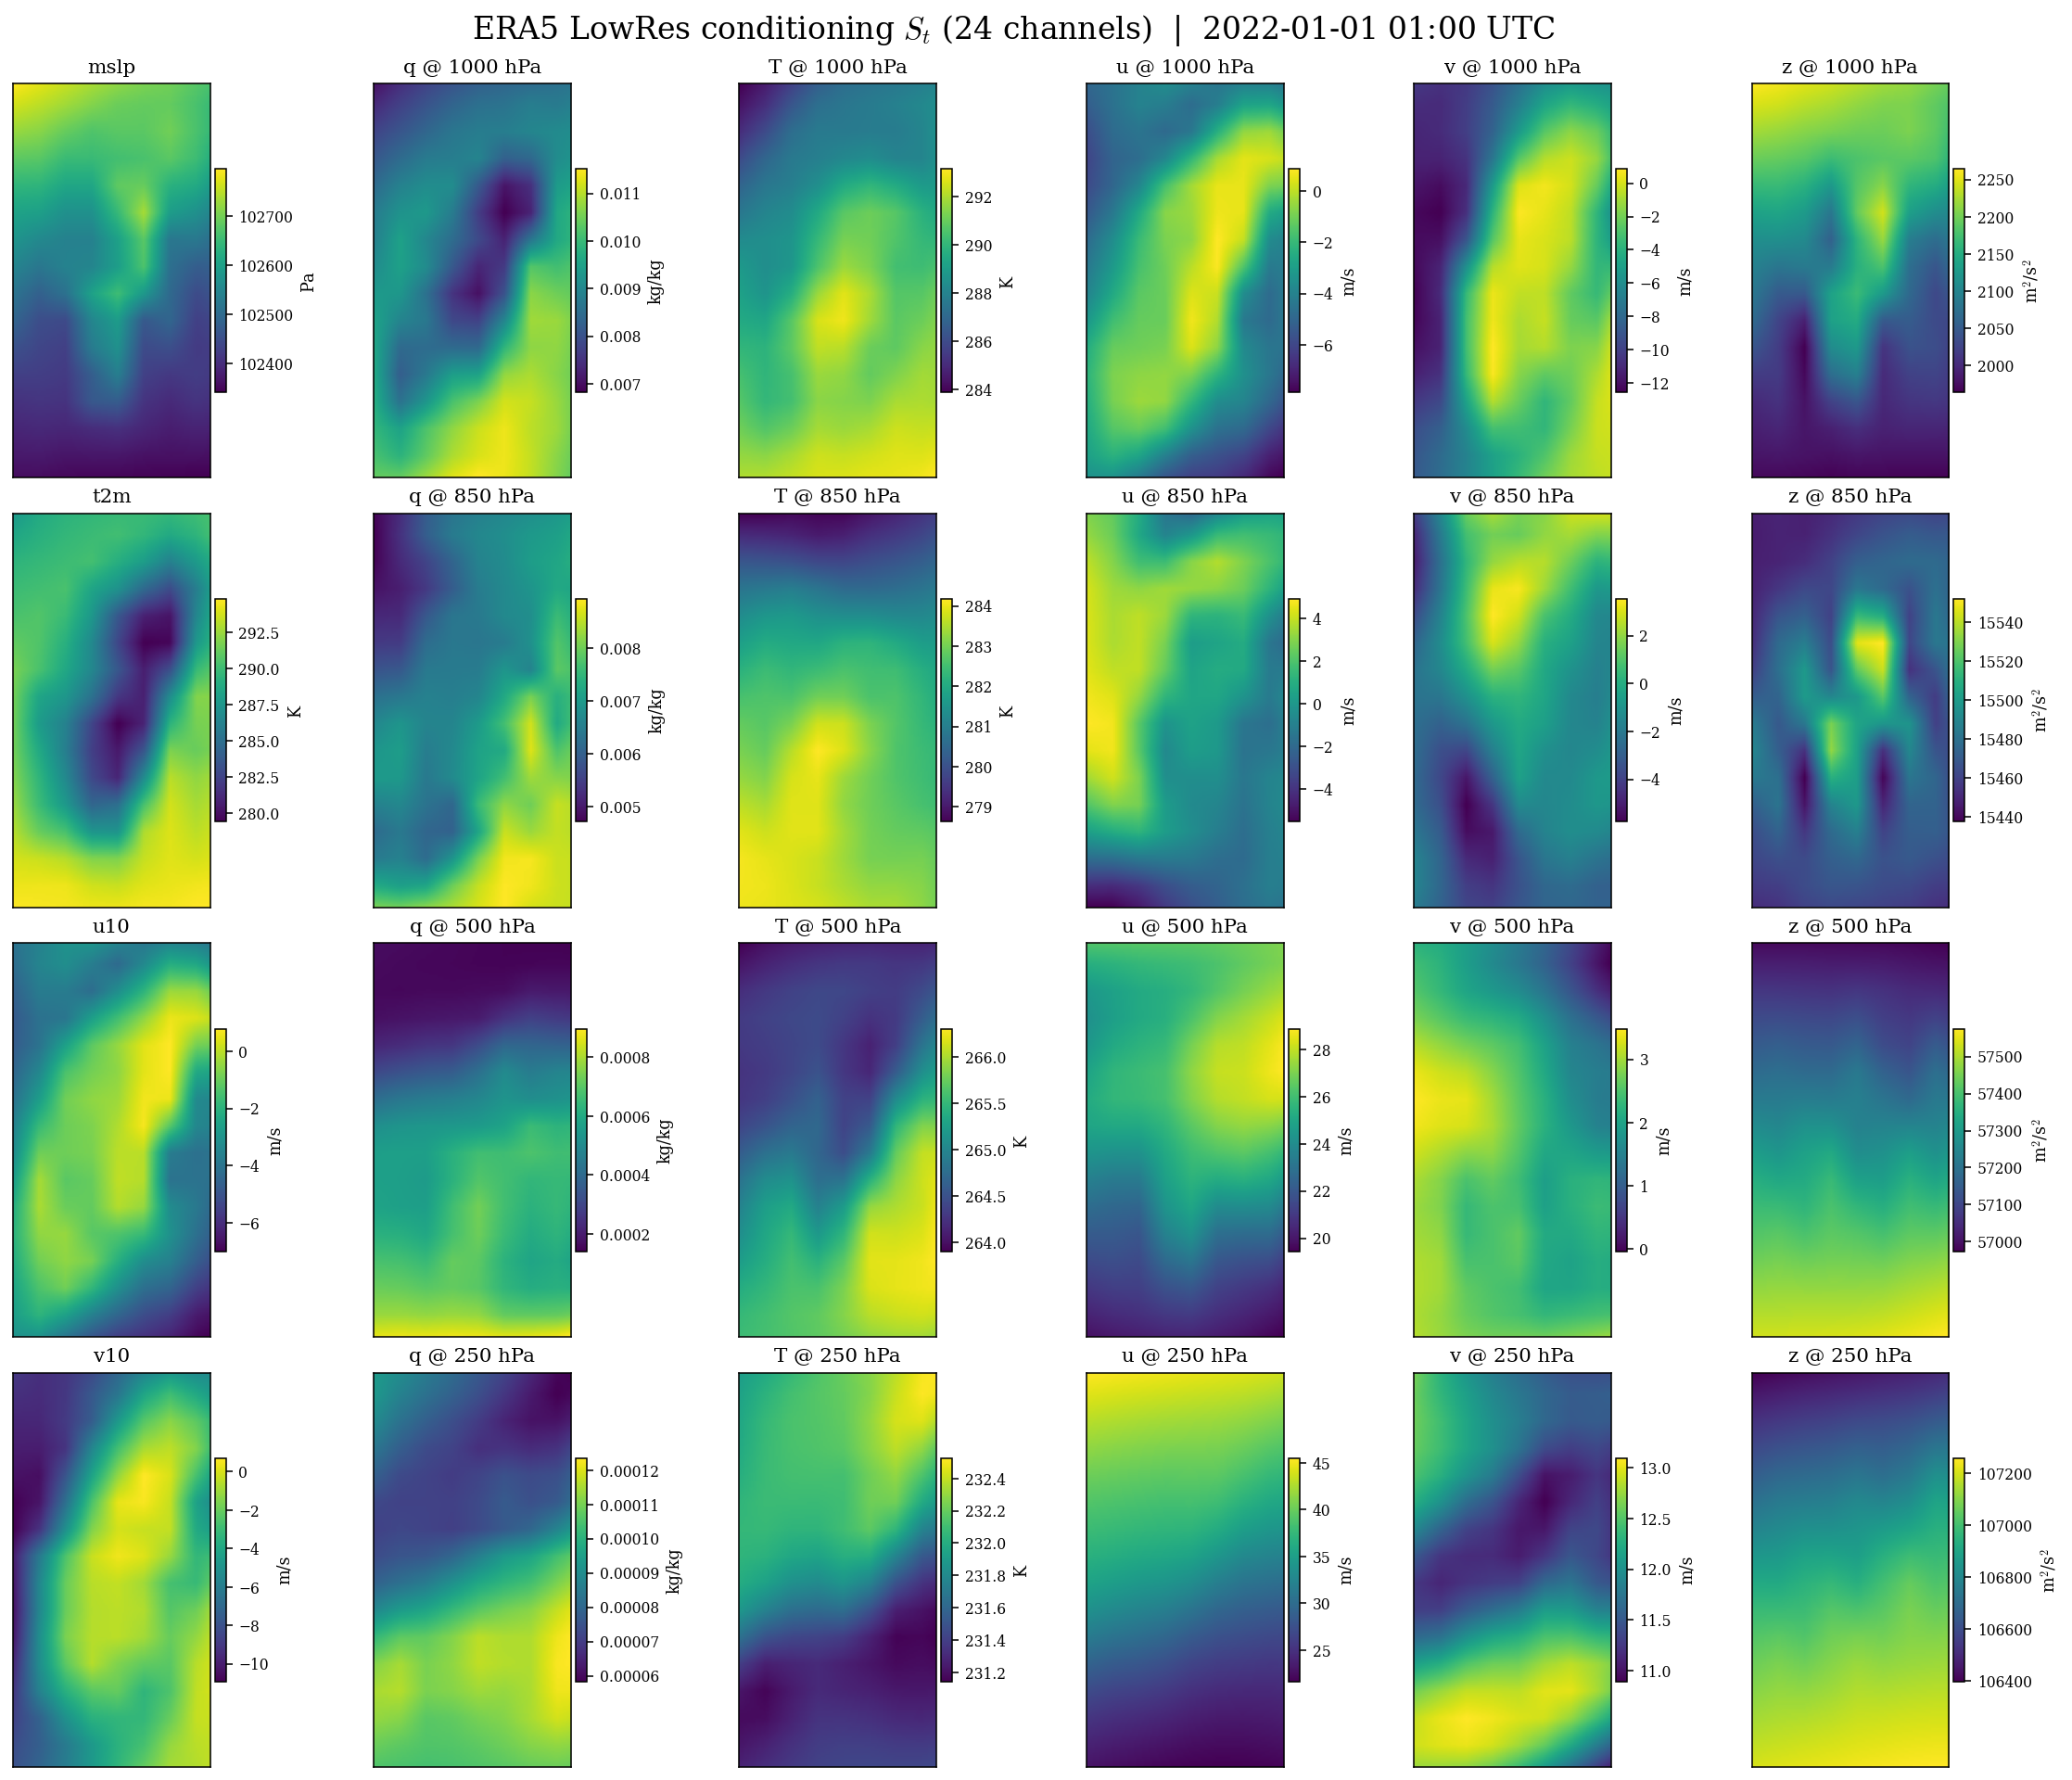
\includegraphics[width=\linewidth]{figures/dataset_losses/era5_lowres.png}
  \caption[ERA5 LowRes conditioning input]{The 24-channel ERA5 LowRes
  conditioning state $S_t$ for a single validation hour (2022-01-01 01:00 UTC),
  in physical units. Top row: the four surface variables (mean sea-level
  pressure, two-metre temperature, ten-metre zonal and meridional winds).
  Rows two through six: specific humidity $q$, temperature $T$, and the wind
  components $u$, $v$ together with geopotential height $z$, each shown across
  the four standard pressure levels \SIlist{1000;850;500;250}{\hecto\pascal}.
  These coarse ($\sim$\SI{25}{\kilo\metre}) re-gridded reanalysis fields supply
  the synoptic-scale environment; they enter the residual heads only indirectly,
  through the regression mean. All panels use the \texttt{viridis} colormap with
  per-panel colour limits. Generated by
  \texttt{experiment\_scripts/make\_dataset\_overview\_figures.py}.}
  \label{fig:era5-lowres}
\end{figure}

% -----------------------------------------------------------------------------
% 2. HighRes target X_{t+1}
% -----------------------------------------------------------------------------
\begin{figure}[htbp]
  \centering
  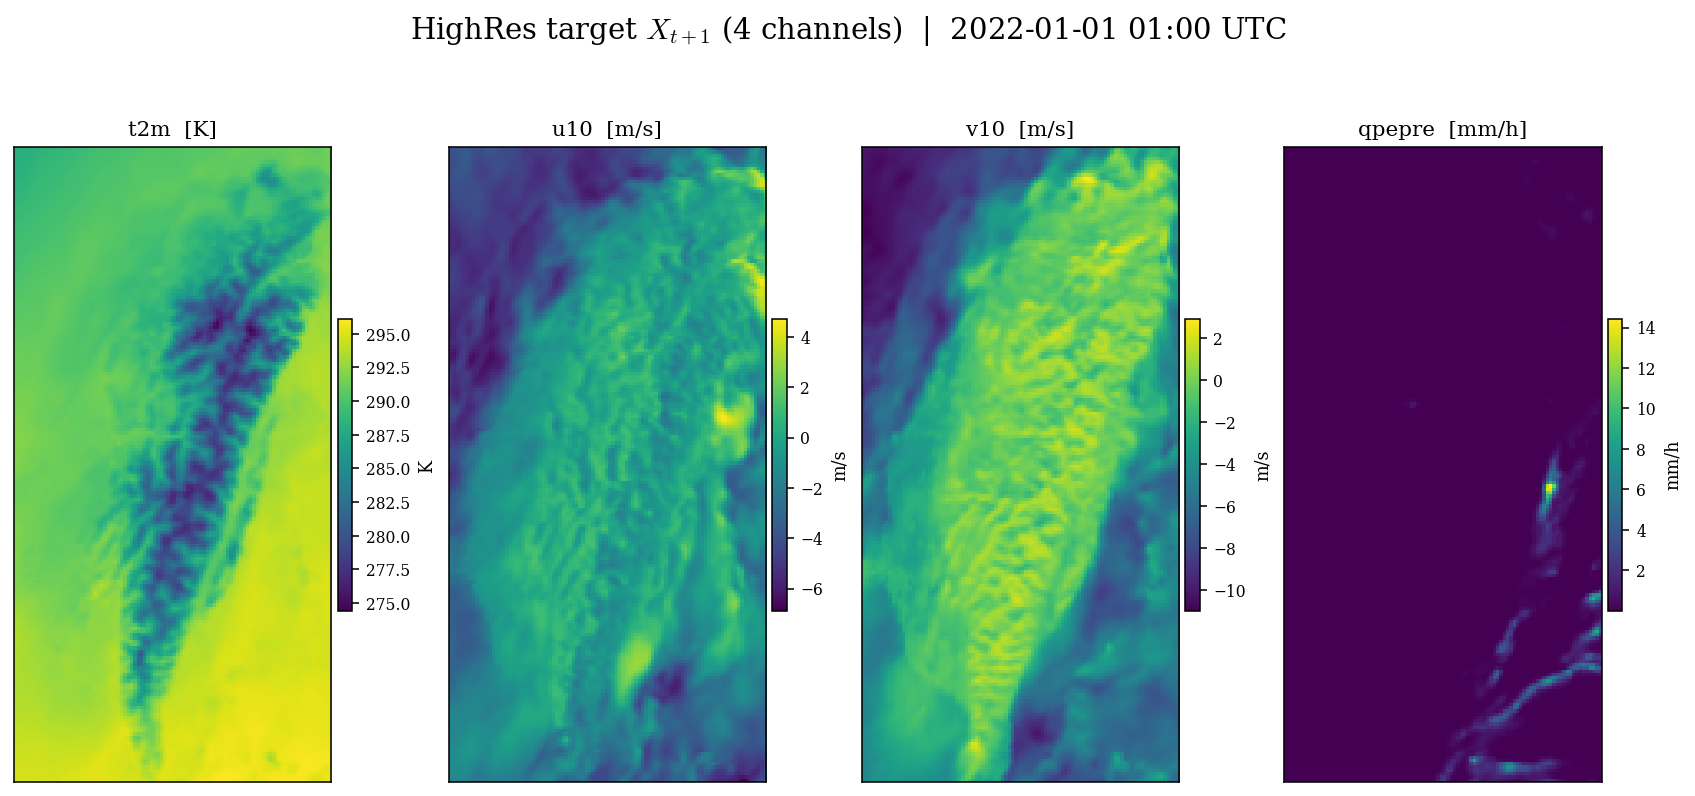
\includegraphics[width=\linewidth]{figures/dataset_losses/highres.png}
  \caption[HighRes target fields]{The four-channel HighRes target $X_{t+1}$ for
  the same validation hour as Figure~\ref{fig:era5-lowres}: two-metre
  temperature \texttt{t2m} (K), ten-metre winds \texttt{u10}, \texttt{v10}
  (m\,s$^{-1}$), and radar-derived hourly precipitation \texttt{qpepre}
  (mm\,h$^{-1}$). The convection-permitting $\sim$\SI{2}{\kilo\metre} grid
  resolves Taiwan's Central Mountain Range (visible as the cold spine in
  \texttt{t2m}) and the sparse, sharp-edged precipitation field that makes
  \texttt{qpepre} the hard channel. This \texttt{qpepre} field is the same one
  shown as ``truth'' in Figure~\ref{fig:method-comparison}. Generated by
  \texttt{experiment\_scripts/make\_dataset\_overview\_figures.py}.}
  \label{fig:highres-target}
\end{figure}

% -----------------------------------------------------------------------------
% 3. Method comparison: StormCast (EDM) vs FlowCast vs MeanFlow
% -----------------------------------------------------------------------------
\begin{figure}[htbp]
  \centering
  \begin{subfigure}[t]{\linewidth}
    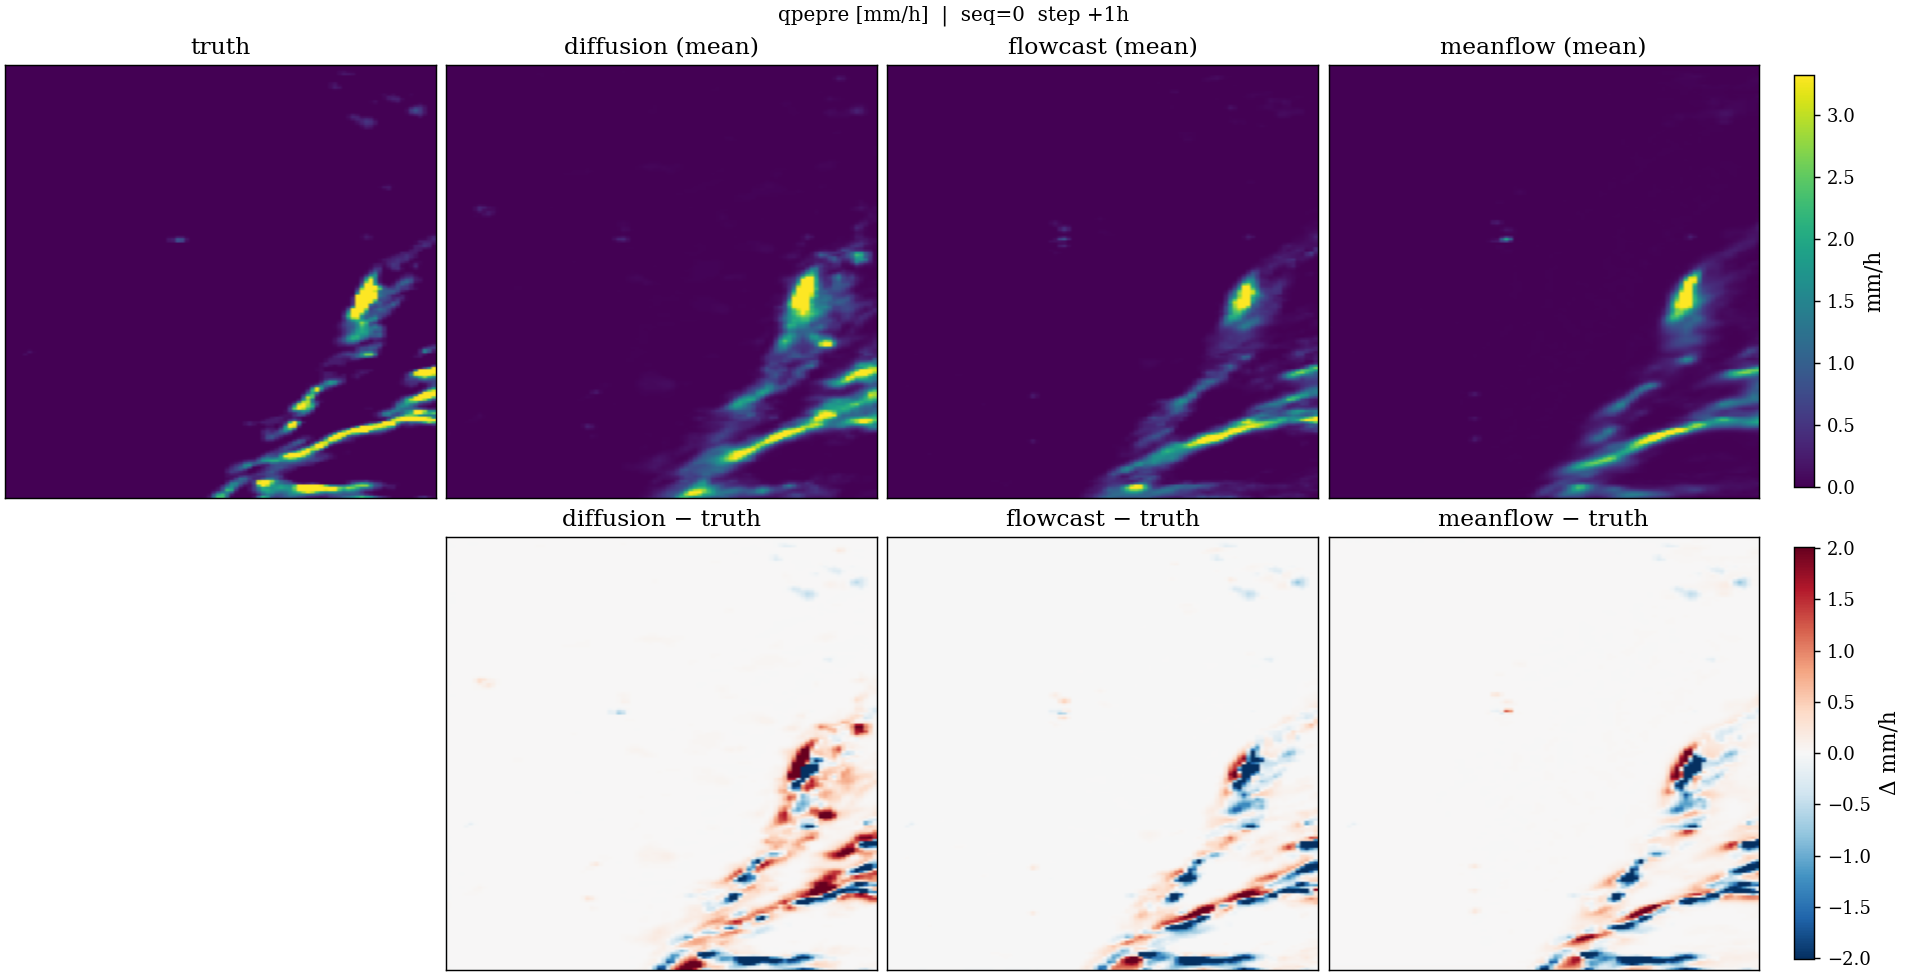
\includegraphics[width=\linewidth]{figures/dataset_losses/method_comparison_qpepre.png}
    \caption{Precipitation \texttt{qpepre} (mm\,h$^{-1}$).}
    \label{fig:method-comparison-qpepre}
  \end{subfigure}

  \vspace{0.8em}
  \begin{subfigure}[t]{\linewidth}
    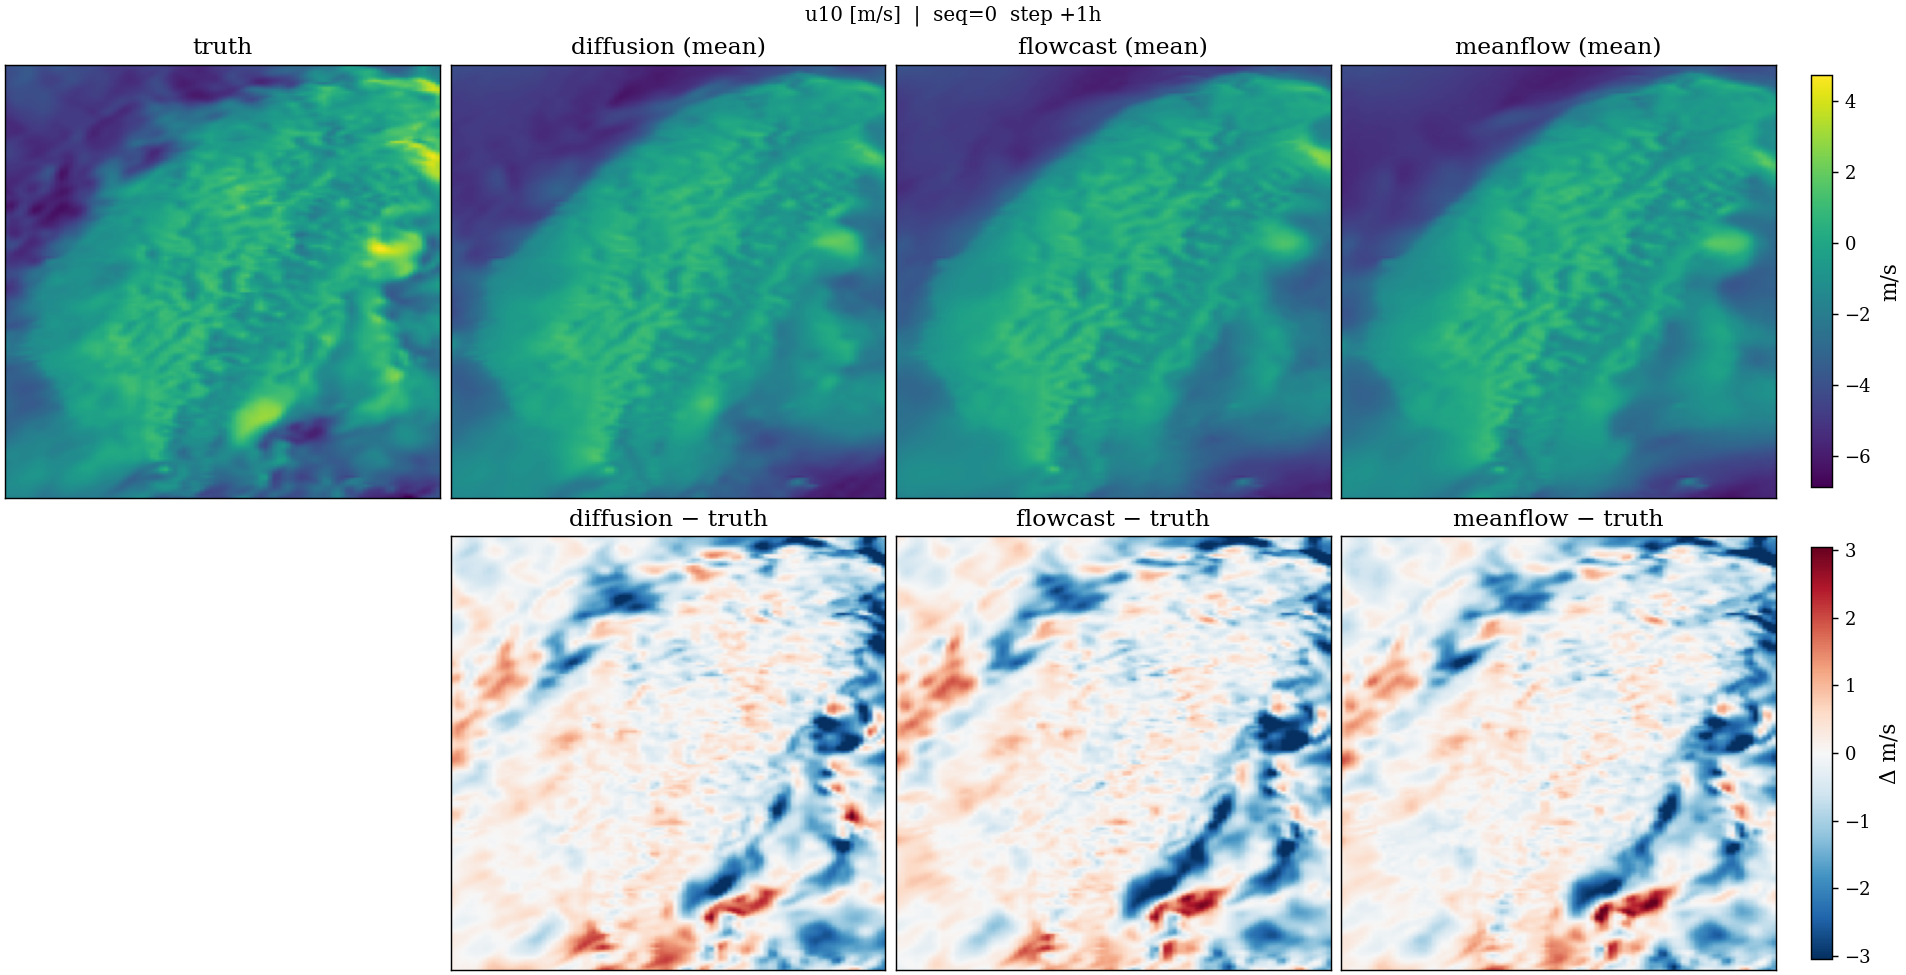
\includegraphics[width=\linewidth]{figures/dataset_losses/method_comparison_u10.png}
    \caption{Ten-metre zonal wind \texttt{u10} (m\,s$^{-1}$).}
    \label{fig:method-comparison-u10}
  \end{subfigure}
  \caption[Qualitative comparison of the three generative heads]{Qualitative
  head-to-head comparison of the three generative residual methods on the
  same +1\,h validation step (2022-01-01 01:00 UTC). In each panel the top row
  shows, left to right, the RWRF/QPEPRE ground truth and the 10-member ensemble
  means of StormCast (the EDM diffusion teacher, labelled \emph{diffusion}),
  FlowCast (CFM student), and MeanFlow (average-velocity student, 1--2 NFE); the
  bottom row shows the corresponding signed error fields (prediction $-$ truth)
  on a diverging scale. All three heads condition on the identical regression
  mean $M_t$, so any difference is attributable to the generative trajectory
  alone. StormCast is the original diffusion baseline; FlowCast and MeanFlow are
  the flow-matching students that match or beat it at a fraction of the
  sampling cost. Field panels use \texttt{viridis}; difference panels use a
  symmetric \texttt{RdBu\_r} scale centred on zero. Generated by
  \texttt{experiment\_scripts/compare\_diffusion\_vs\_flowcast.py}.}
  \label{fig:method-comparison}
\end{figure}

% =============================================================================

% -----------------------------------------------------------------------------
% 1. ERA5 LowRes conditioning input S_t
% -----------------------------------------------------------------------------
\begin{figure}[htbp]
  \centering
  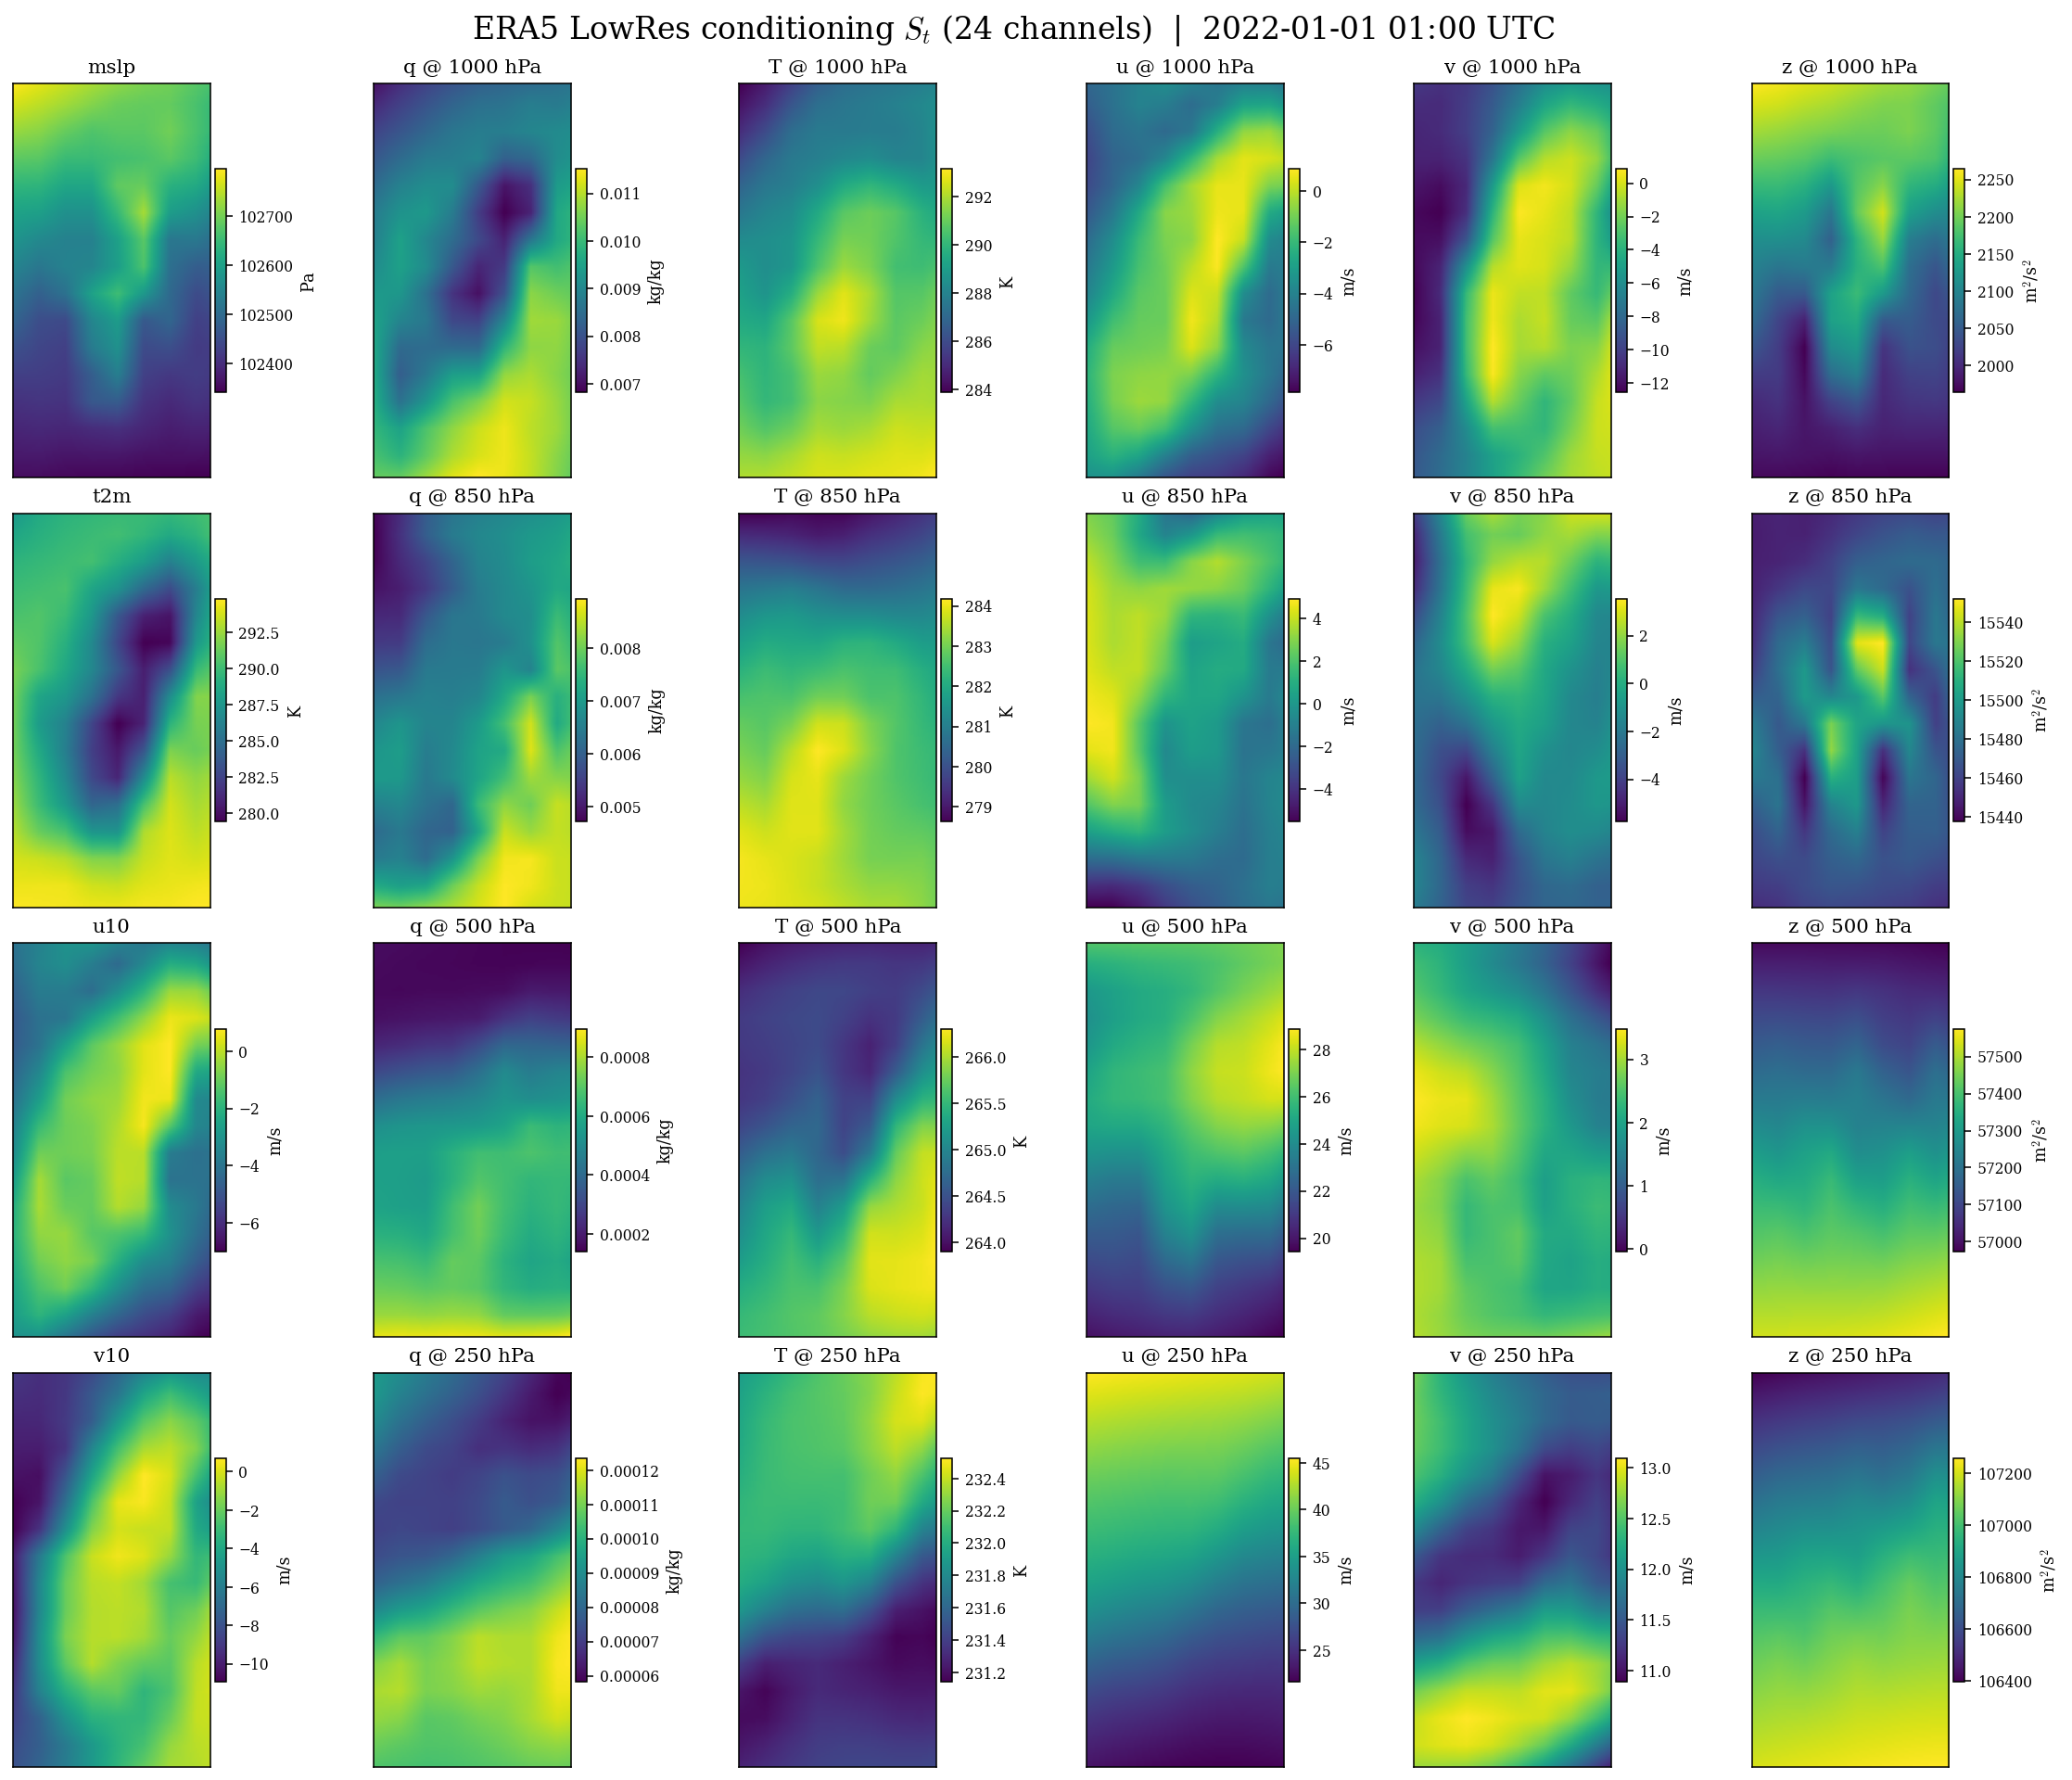
\includegraphics[width=\linewidth]{figures/dataset_losses/era5_lowres.png}
  \caption[ERA5 LowRes conditioning input]{The 24-channel ERA5 LowRes
  conditioning state $S_t$ for a single validation hour (2022-01-01 01:00 UTC),
  in physical units. Top row: the four surface variables (mean sea-level
  pressure, two-metre temperature, ten-metre zonal and meridional winds).
  Rows two through six: specific humidity $q$, temperature $T$, and the wind
  components $u$, $v$ together with geopotential height $z$, each shown across
  the four standard pressure levels \SIlist{1000;850;500;250}{\hecto\pascal}.
  These coarse ($\sim$\SI{25}{\kilo\metre}) re-gridded reanalysis fields supply
  the synoptic-scale environment; they enter the residual heads only indirectly,
  through the regression mean. All panels use the \texttt{viridis} colormap with
  per-panel colour limits. Generated by
  \texttt{experiment\_scripts/make\_dataset\_overview\_figures.py}.}
  \label{fig:era5-lowres}
\end{figure}

% -----------------------------------------------------------------------------
% 2. HighRes target X_{t+1}
% -----------------------------------------------------------------------------
\begin{figure}[htbp]
  \centering
  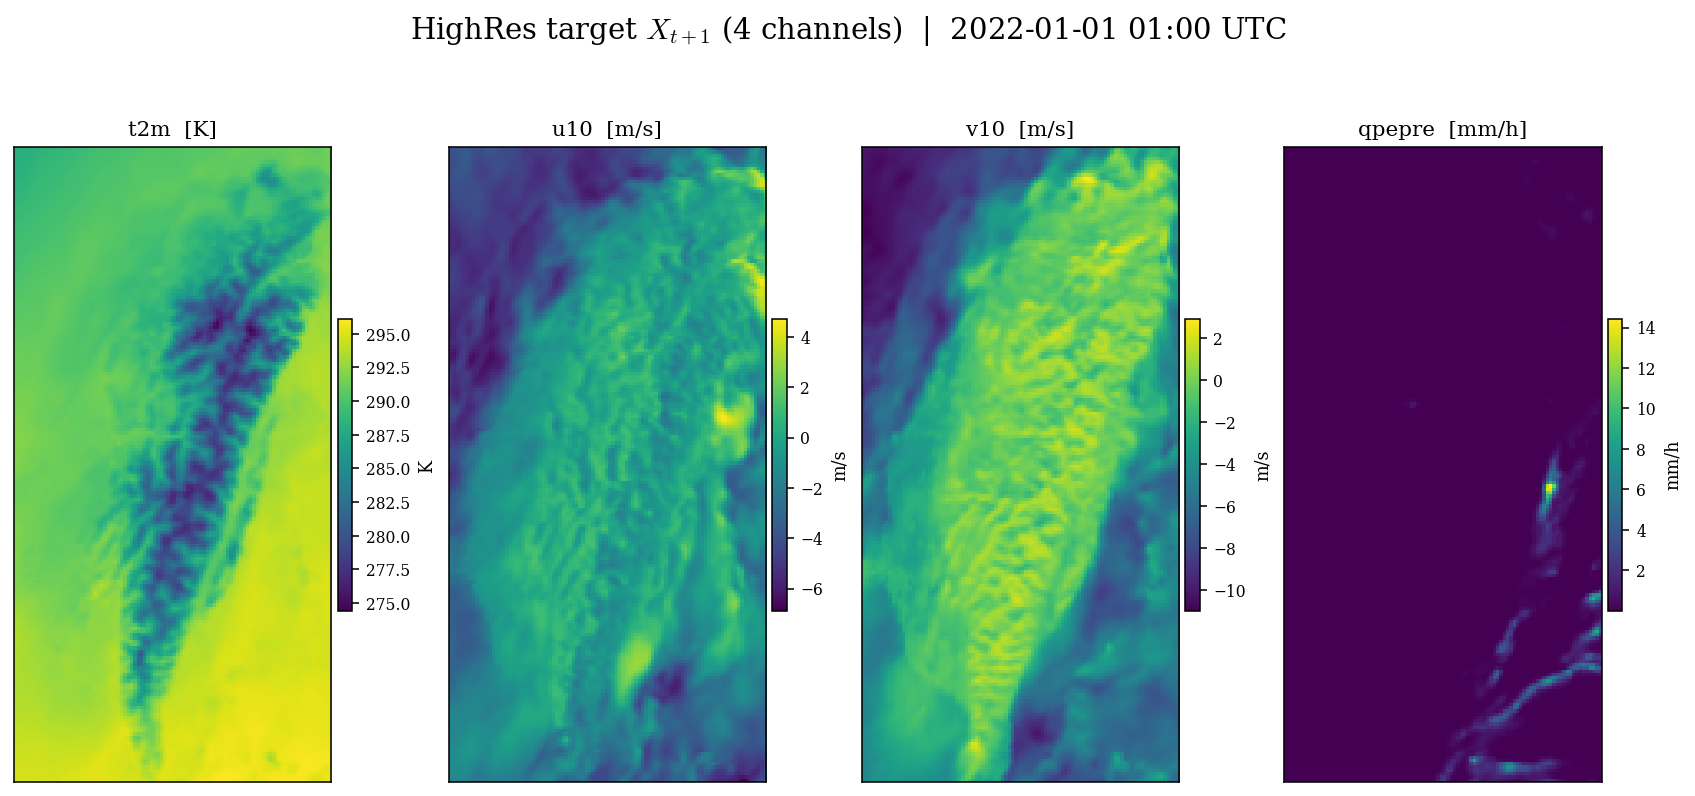
\includegraphics[width=\linewidth]{figures/dataset_losses/highres.png}
  \caption[HighRes target fields]{The four-channel HighRes target $X_{t+1}$ for
  the same validation hour as Figure~\ref{fig:era5-lowres}: two-metre
  temperature \texttt{t2m} (K), ten-metre winds \texttt{u10}, \texttt{v10}
  (m\,s$^{-1}$), and radar-derived hourly precipitation \texttt{qpepre}
  (mm\,h$^{-1}$). The convection-permitting $\sim$\SI{2}{\kilo\metre} grid
  resolves Taiwan's Central Mountain Range (visible as the cold spine in
  \texttt{t2m}) and the sparse, sharp-edged precipitation field that makes
  \texttt{qpepre} the hard channel. This \texttt{qpepre} field is the same one
  shown as ``truth'' in Figure~\ref{fig:method-comparison}. Generated by
  \texttt{experiment\_scripts/make\_dataset\_overview\_figures.py}.}
  \label{fig:highres-target}
\end{figure}

% -----------------------------------------------------------------------------
% 3. Method comparison: StormCast (EDM) vs FlowCast vs MeanFlow
% -----------------------------------------------------------------------------
\begin{figure}[htbp]
  \centering
  \begin{subfigure}[t]{\linewidth}
    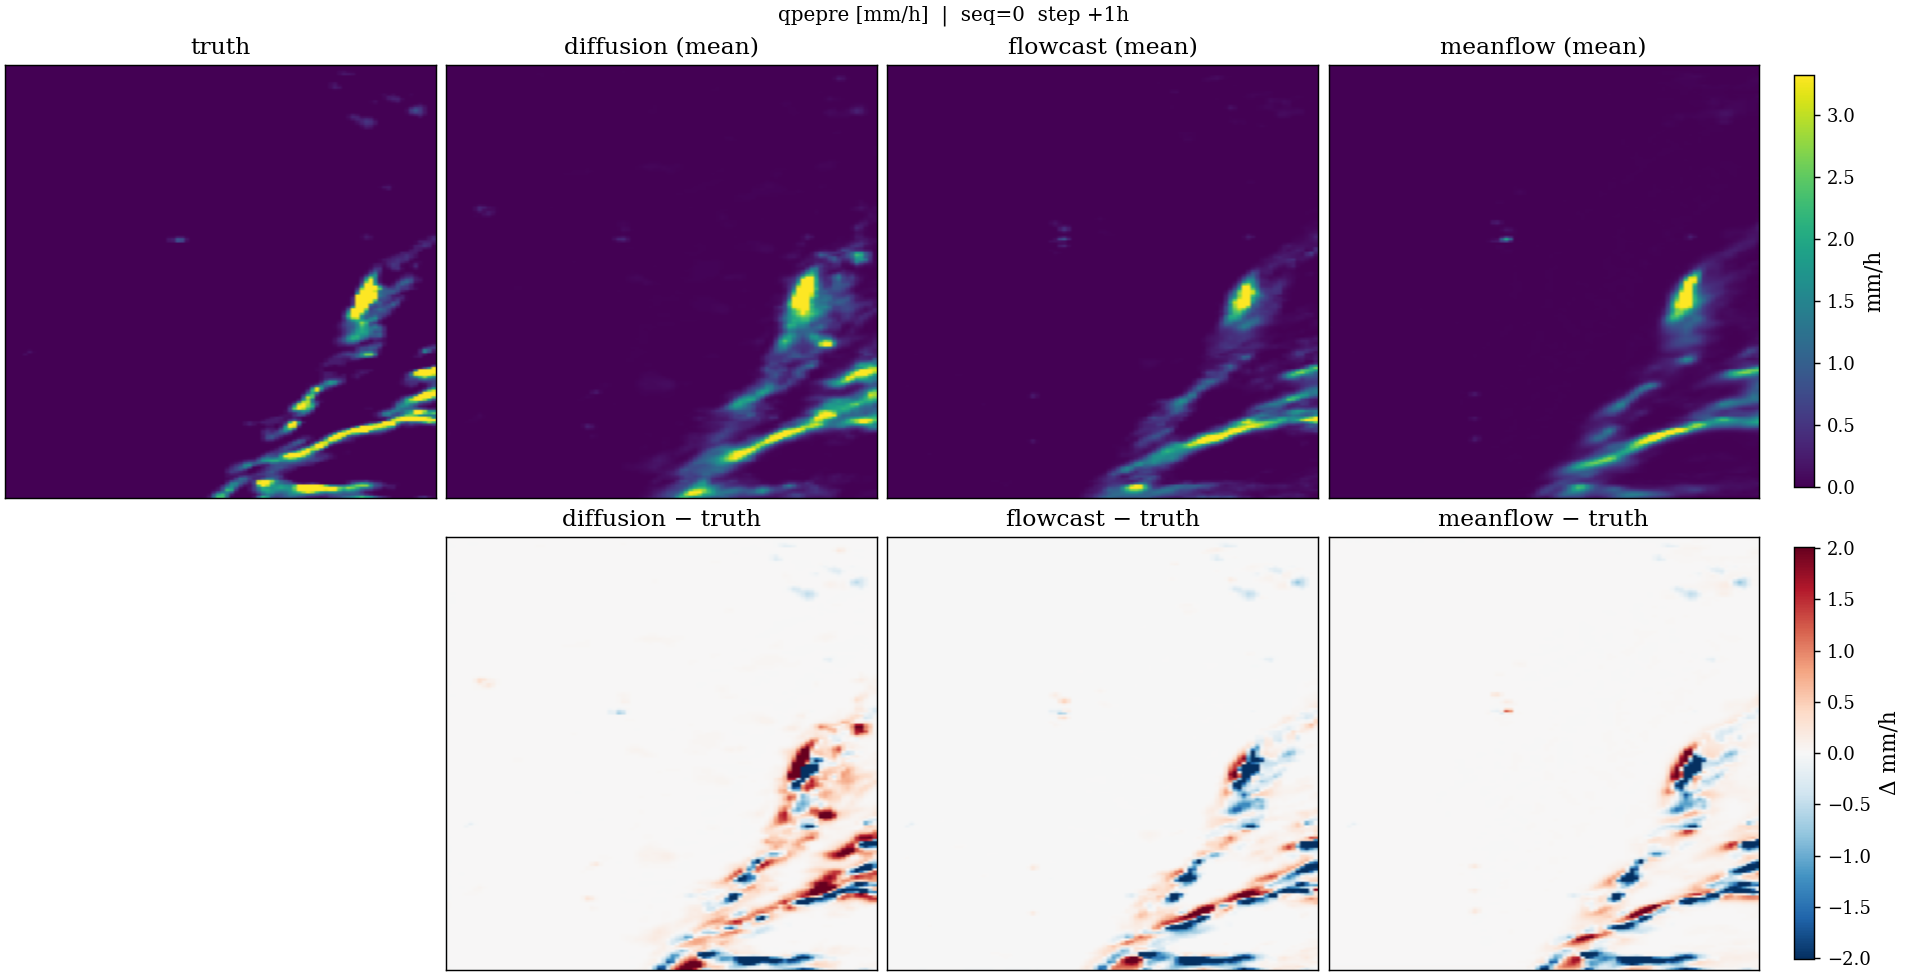
\includegraphics[width=\linewidth]{figures/dataset_losses/method_comparison_qpepre.png}
    \caption{Precipitation \texttt{qpepre} (mm\,h$^{-1}$).}
    \label{fig:method-comparison-qpepre}
  \end{subfigure}

  \vspace{0.8em}
  \begin{subfigure}[t]{\linewidth}
    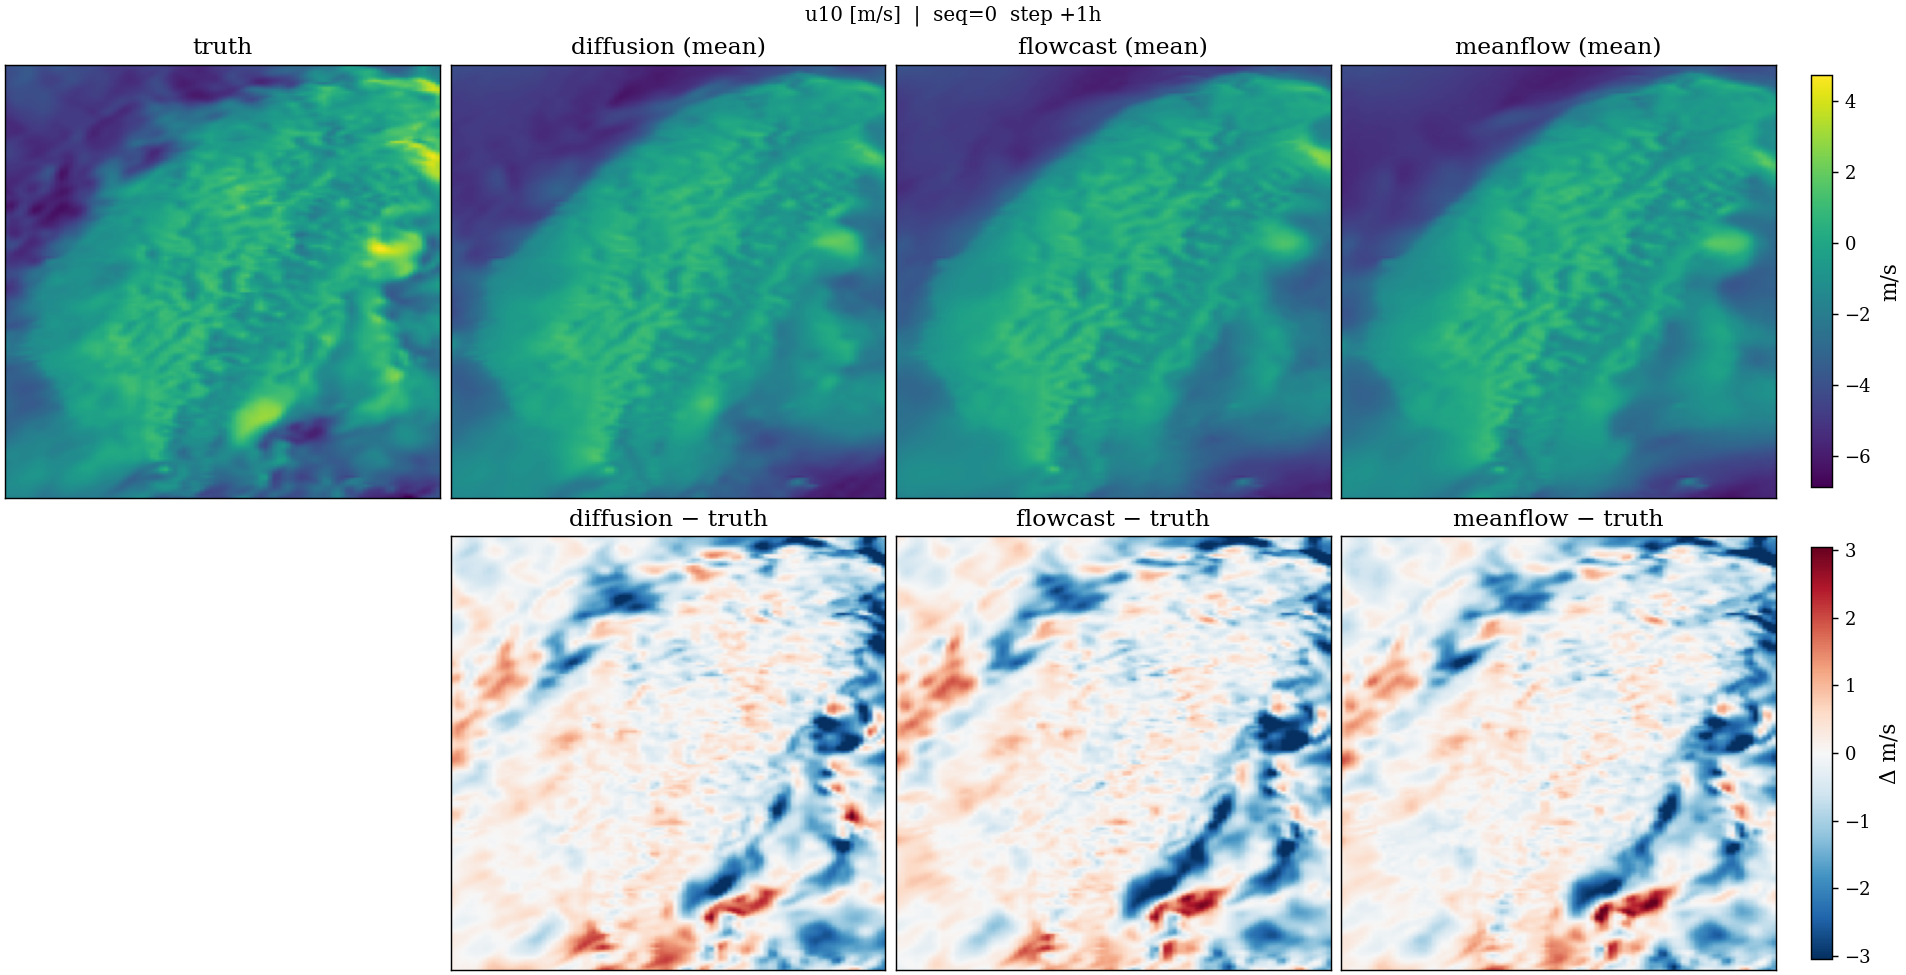
\includegraphics[width=\linewidth]{figures/dataset_losses/method_comparison_u10.png}
    \caption{Ten-metre zonal wind \texttt{u10} (m\,s$^{-1}$).}
    \label{fig:method-comparison-u10}
  \end{subfigure}
  \caption[Qualitative comparison of the three generative heads]{Qualitative
  head-to-head comparison of the three generative residual methods on the
  same +1\,h validation step (2022-01-01 01:00 UTC). In each panel the top row
  shows, left to right, the RWRF/QPEPRE ground truth and the 10-member ensemble
  means of StormCast (the EDM diffusion teacher, labelled \emph{diffusion}),
  FlowCast (CFM student), and MeanFlow (average-velocity student, 1--2 NFE); the
  bottom row shows the corresponding signed error fields (prediction $-$ truth)
  on a diverging scale. All three heads condition on the identical regression
  mean $M_t$, so any difference is attributable to the generative trajectory
  alone. StormCast is the original diffusion baseline; FlowCast and MeanFlow are
  the flow-matching students that match or beat it at a fraction of the
  sampling cost. Field panels use \texttt{viridis}; difference panels use a
  symmetric \texttt{RdBu\_r} scale centred on zero. Generated by
  \texttt{experiment\_scripts/compare\_diffusion\_vs\_flowcast.py}.}
  \label{fig:method-comparison}
\end{figure}
